\documentclass{aghdpl}

\usepackage[polish]{babel}
\usepackage[utf8]{inputenc}

% dodatkowe pakiety
%\usepackage{apacite}
\usepackage{enumerate}
\usepackage{listings}
\usepackage{textcomp}
\usepackage{graphics}
\usepackage[hang, font={large, sl}, labelfont={large, sl}]{caption}
\usepackage{amsthm}
\usepackage{multirow} 
\usepackage{tocloft}
\usepackage{setspace}
\usepackage{url}
\usepackage{pdfpages}

% \setcounter{secnumdepth}{0}
\setcounter{chapter}{0}
\renewcommand\cfttoctitlefont{\Large\bfseries}
\renewcommand\cftchapfont{\Large\bfseries}
\renewcommand\cftsecfont{\Large}
\renewcommand\cftsubsecfont{\large}

\renewcommand\cftchappagefont{\Large\bfseries}
\renewcommand\cftsecpagefont{\Large}
\renewcommand\cftsubsecpagefont{\large}

\renewcommand\cftchapafterpnum{\par\addvspace{11pt}}
\renewcommand\cftsecafterpnum{\par\addvspace{8pt}}
\renewcommand\cftsubsecafterpnum{\par\addvspace{6pt}}

\renewcommand\cftloftitlefont{\LARGE\bfseries}
\renewcommand\cftfigfont{\large}
\renewcommand\cftfigpagefont{\large}
\renewcommand\cftfigafterpnum{\par\addvspace{0pt}}

\setlength{\cftfignumwidth}{3em}

\lstloadlanguages{TeX}

\lstset{
  literate={ą}{{\k{a}}}1
           {ć}{{\'c}}1
           {ę}{{\k{e}}}1
           {ó}{{\'o}}1
           {ń}{{\'n}}1
           {ł}{{\l{}}}1
           {ś}{{\'s}}1
           {ź}{{\'z}}1
           {ż}{{\.z}}1
           {Ą}{{\k{A}}}1
           {Ć}{{\'C}}1
           {Ę}{{\k{E}}}1
           {Ó}{{\'O}}1
           {Ń}{{\'N}}1
           {Ł}{{\L{}}}1
           {Ś}{{\'S}}1
           {Ź}{{\'Z}}1
           {Ż}{{\.Z}}1
}

%---------------------------------------------------------------------------

\author{Damian Burek}
\shortauthor{D. Burek}

\titlePL{Przenośny układ do nieinwazyjnego pomiaru wysycenia krwi tętniczej i częstości akcji serca}
\titleEN{A portable device for noninvasive measurement of oxygen saturation in blood and heart rate}

\shorttitlePL{} % skrócona wersja tytułu jeśli jest bardzo długi
\shorttitleEN{}

\thesistypePL{Praca magisterska}
\thesistypeEN{Master of Science Thesis}

\supervisorPL{dr inż. Wojciech Maziarz}
\supervisorEN{Wojciech Maziarz Ph.D.}

\date{2013}

\departmentPL{Katedra Elektroniki}
\departmentEN{Department of Electronics}

\facultyPL{Wydział Informatyki, Elektroniki i Telekomunikacji}
\facultyEN{Faculty of Computer Science, Electronics and Telecommunications}

\acknowledgements{}

\setlength{\cftsecnumwidth}{10mm}

%---------------------------------------------------------------------------

\begin{document}

\titlepages

\tableofcontents

\clearpage
\linespread{2}


\renewcommand{\figurename}{Rys.}

\chapter*{Wprowadzenie}
\label{cha:wprowadzenie}
\addcontentsline{toc}{chapter}{Wprowadzenie}

\section*{Podstawowe parametry życiowe}
\label{sec:ParametryZyciowe}
\addcontentsline{toc}{section}{Podstawowe parametry życiowe}

\fontsize{14}{15}\selectfont

Monitorowanie stanu pacjentów jest istotnym elementem opieki pielęgniarskiej i~anestezjologicznej, gdyż dostarcza podstawowych 
informacji na temat bieżącej kondycji organizmu. Rejestracja podstawowych parametrów ustroju jest prowadzona w~sposób ciągły 
na oddziałach intensywnej terapii, chirurgii, pediatrii i~podczas przeprowadzania prób wysiłkowych w~kardiologii oraz medycynie 
sportowej. Systematyczny monitoring wybranych parametrów, umożliwia natychmiastowe wykrycie odchyleń wskaźników od norm, co 
może być oznaką pogorszenia stanu zdrowia lub zagrożenia życia pacjenta. Parametry te to m.in.:

\begin{itemize}
	\item temperatura
	\item częstość akcji serca
	\item częstość oddechów
	\item ciśnienie tętnicze krwi
	\item wysycenie krwi tlenem.
\end{itemize}

Pomiar temperatury, dokonywany poprzez umieszczenie~w ustach, uchu lub dole pachowym termometru, pozwala na zidentyfikowanie gorączki, 
hipotermii (obniżenia temperatury ciała) oraz ich wykluczenie, poprzez stwierdzenie normy. W zależności od miejsca pomiaru temperatury 
otrzymuje się wartości, których średnia wynosi: 36,8\textdegree~C~\cite{SzGa11}.\\

Tętno, czyli częstość skurczów serca na minutę, to rytmiczne rozciąganie naczyń krwionośnych wywołane nagłymi zmianami ciśnienia krwi 
w~następstwie skurczów i~rozkurczów komór serca. Można je mierzyć palpacyjnie, poprzez uciśnięcie danej tętnicy i~liczenie ilości uderzeń 
fal tętna lub za pomocą urządzeń rejestrujących tętno z~elektrod EKG i~pulsoksymetru.
Częstotliwość tętna u~człowieka zależy od wieku, wysiłku fizycznego, stanów emocjonalnych, choroby. W~wieku dojrzałym wynosi średnio 72 
uderzenia na minutę, w~wieku starszym średnio 67~\cite{SzGa11}.\\

Proces wymiany gazowej ustroju polega na dostarczaniu komórkom tlenu i~wydalaniu na zewnątrz dwutlenku węgla. Częstotliwość oddechów to liczba 
uniesień klatki piersiowej w~ciągu określonego przedziału czasu, najczęściej 60 sekund.
Częstość oddychania u~ludzi zdrowych wynosi 16-18 razy na 1 minutę u~dorosłych, 20-30 razy u~dzieci, 30-35 u~noworodka~\cite{SzGa11}. W~warunkach 
fizjologicznych na zmianę szybkości oddychania wpływa wzmożony wysiłek fizyczny, stany emocjonalne. W~warunkach patologicznych na przyspieszenie 
oddychania wpływają: stany gorączkowe, bolesne urazy, zabiegi operacyjne.\\

Ciśnienie tętnicze to ciśnienie wywierane przez krew na ścianki tętnic, przy czym rozumie się pod tą nazwą ciśnienie w~największych tętnicach, 
np.~w~tętnicy w~ramieniu. W~momencie skurczu serca, kiedy porcja krwi wypychana jest z~serca do aorty, w~tętnicach panuje najwyższe ciśnienie, 
wynoszące zazwyczaj u~zdrowego dorosłego człowieka od ok. 90 do 135 mmHg. W~chwili rozkurczu wartość ciśnienia krwi jest najniższa, np.~od ok. 50 
do 90~mmHg~\cite{SzGa11}. Pomiarów zazwyczaj dokonuje się metodą Korotkowa, przy użyciu sfigmomanometru i~słuchawek lekarskich, bądź metodami półautomatycznymi.\\

Saturacja oznacza nasycenie cieczy gazem. W~medycynie dokonuje się pomiarów nasycenia płynów ustrojowych, m.in.~krwi czy płynu komórkowego, gazami.
Najbardziej powszechnym pomiarem saturacji w~działaniach medycznych jest pomiar nasycenia krwi tętniczej tlenem metodą pulsoksymetrii w~celu 
przeciwdziałania niewydolności oddechowej. Pomiar wyznacza stopień wiązania hemoglobiny we krwi z~tlenem (zawartości oksyhemoglobiny). Wartość 
saturacji krwi tlenem u zdrowych ludzi zawiera się w~zakresie SpO2 95\%~–~99\%~\cite{SzGa11}. Saturacja poniżej 90\% oznacza niedotlenienie, 
które może być spowodowane m.in. przez niedokrwistość (anemię).\\

Rozpoznawanie i~ocena zjawisk fizjologicznych i~patologicznych towarzyszących zabiegom operacyjnym i~terapeutycznym oraz procesom chorobowym wymagają 
ciągłego lub powtarzalnego w~określonych odstępach czasu monitorowania wszystkich podstawowych parametrów życiowych. W~skład standardowego 
stanowiska anestezjologicznego wchodzą urządzenia umożliwiające pomiar i~obrazowanie powyższych wskaźników zintegrowane w~centralny monitor 
pacjenta~(rys. \ref{rys:central_monitor}).
\begin{figure}[!h]
	\centerline{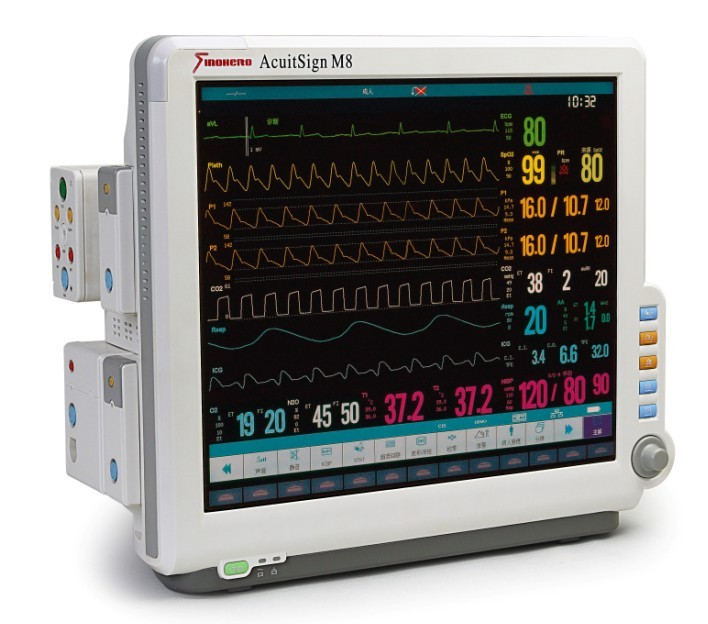
\includegraphics[scale = 0.45]{graphic/patient_monitor.jpg}}
	\caption{Centralny monitor pacjenta}
	~\\	 
	(źródło: http://www.axmeditec.com.pl)
	\label{rys:central_monitor}
\end{figure}

%---------------------------------------------------------------------------
\section*{Nieinwazyjne metody rejestracji sygnałów biomedycznych}
\label{sec:MetodyPomiarow}
\addcontentsline{toc}{section}{Nieinwazyjne metody rejestracji sygnałów biomedycznych.}

Istnieją różne sposoby ratowania i~ochrony życia. Aby określić najlepszą metodę leczenia pacjentów, specjaliści muszą wziąć pod uwagę różnorodne 
czynniki. Obok perspektywy medyczno-terapeutycznej dużą rolę odgrywa też fizyczna i~psychiczna presja wywierana na pacjenta podczas leczenia, 
jak również czas wymagany do zastosowania danego środka. Celem jest osiągnięcie jak najszybszego i~bezproblemowego procesu leczenia, przy czym 
ważną rolę odgrywają również aspekty ekonomiczne, które należy wziąć pod uwagę podczas wyboru odpowiedniej procedury diagnostycznej i~terapeutycznej. 
Zastosowanie nieinwazyjnych technologii może przyczynić się do zwiększenia dobrego samopoczucia pacjenta oraz uniknięcia powikłań podczas leczenia.

Nieinwazyjne metody monitorowania pacjenta są szybkie i~oszczędne. Ponadto są one najbardziej atrakcyjną alternatywą dla pacjentów i~mogą pomóc 
w~unikaniu infekcji. Przyczyną tego jest fakt, że każda ingerencja w~ciało, np. przy użyciu igieł lub cewników, otwiera szeroko drzwi infekcjom. 
W~sytuacji, która i~tak jest już stresująca dla pacjenta, pomiary inwazyjne zazwyczaj powodują dodatkowy ból i~stres.

Współczesne techniki obrazowania wykorzystują szereg zjawisk fizycznych umożliwiających nieinwazyjną rejestrację biosygnałów bez konieczności 
ingerencji chirurgicznej. Interakcja fali mechanicznej w~postaci ultradźwięków, pola magnetycznego oraz szerokiego zakresu promieniowania 
elektromagnetycznego~(rys. \ref{rys:spectrum}) z~ustrojem, stanowi bogate źródło użytecznych sygnałów, niosących istotne informacje na temat 
formy i~kondycji organizmu.
\begin{figure}[!h]
	\centerline{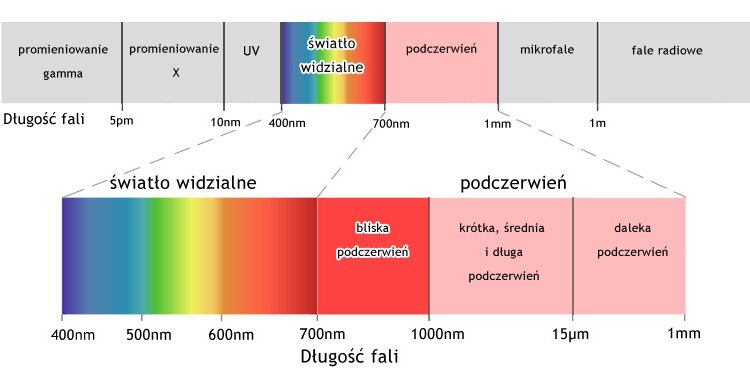
\includegraphics[scale = 0.56]{graphic/spectrum.jpg}}
	\caption{Spektrum fal elektromagnetycznych}
	~\\	
	(źródło: http://www.zebu.uoregon.edu)
	\label{rys:spectrum}
\end{figure}

\noindent Do najczęściej stosowanych metod obrazowania oraz diagnostyki w~praktyce medycznej należą~\cite{SzGa11}:
\begin{itemize}
	\item pulsoksymetria
	\item rentgenografia i~mammografia (RTG)
	\item ultrasonografia (USG)
	\item tomografia komputerowa (CT)
	\item tomografia rezonansu magnetycznego (MRT)
	\item pozytonowa tomografia emisyjna (PET)
	\item optyczna tomografia koherencyjna (OCT).\\
\end{itemize}

Wraz z~dynamicznym rozwojem technologii oraz tendencją do miniaturyzacji urządzeń i~przyrządów elektronicznych, pojawia się szereg nowych możliwości
i~perspektyw związanych z~obszarem obrazowania medycznego. Spośród różnorodnych usług realizowanych przez systemy telemedyczne, szczególnie istotną 
rolę odgrywa zdalne monitorowanie stanu pacjenta w~zakresie śledzenia wybranych parametrów i~sygnałów fizjologicznych. Temperatura, tętno, saturacja
czy ciśnienie krwi to wskaźniki, których wartości mogą być śledzone w~sposób ciągły w~trakcie wykonywania codziennych czynności i~podczas snu, nie 
wprowadzając dyskomfortu podczas ich rejestracji. 
%---------------------------------------------------------------------------

\section*{Cel i~zakres pracy}
\label{sec:celePracy}
\addcontentsline{toc}{section}{Cel i~zakres pracy}

Celem pracy magisterskiej jest zaprojektowanie oraz sprzętowa realizacja przenośnego układu do pomiaru wysycenia krwi tętniczej tlenem 
i~częstości akcji serca. Ponadto praca ma na celu przedstawienie podstawowych właściwości i~zjawisk optycznych dotyczących zbiorów tkanek 
oraz ich znaczenie w pomiarach parametrów układu krążeniowo~-~oddechowego. Bazując na analizie różnic w widmach absorpcyjnych składników
krwi przedstawiona zostanie metodyka wyznaczania parametrów krwi tętniczej, określających stan i kondycję organizmu oraz ich znaczenie fizjologiczne.

Budowa aparatu pomiarowego, którego zasada działania oparta będzie o detekcję oraz analizę sygnałów optycznych uzyskanych w~procesie 
transluminacji wymaga realizacji analogowego toru przetwarzania sygnału wraz z cyfrową częścią sterującą w~postaci układu mikroprocesorowego. 
Docelowa lokalizacja przeprowadzania testów i~pomiarów to końcówki palców dłoni charakteryzujące się silnym unaczynnieniem.\\ 

\noindent Wymagania dotyczące sprzętowej realizacji układu pulsoksymetru:
\begin{itemize}
	\item Stworzenie schematu elektrycznego analogowego toru przetwarzania wraz z~cyfrową częścią sterującą;
	\item Zaprojektowanie i~wykonanie układu pomiarowego w~formie obwodu drukowanego PCB;
	\item Dobór odpowiednich elementów i~podzespołów elektronicznych pulsoksymetru i~sondy pomiarowej;
	\item Stworzenie kodu aplikacji kontrolnej mikrokontrolera, sterującej procesem pomiarowym (np.~ANSI~C);
	\item Umożliwienie wizualizacji wyników na komputerze PC z aplikacją LabView, ewentualnie za pomocą dedykowanego wyświetlacza LCD;
	\item Zaplanowanie oraz wykonanie serii testów i~pomiarów, weryfikujących stopień poprawności uzyskanych wyników.
\end{itemize}
%---------------------------------------------------------------------------


\renewcommand{\figurename}{Rys.}

\chapter{Właściwości optyczne tkanek}
\label{cha:WlasciowosciOptyczne}

\fontsize{14}{15}\selectfont
%---------------------------------------------------------------------------

Selektywne właściwości optyczne tkanek umożliwiają określanie istotnych cech zbiorów komórek przy zastosowaniu
optoelektronicznych metod pomiarowych, szczególnie przydatnych w~diagnostyce nieinwazyjnej. Wśród stosowanych sposobów 
pomiaru parametrów tkanek, wyróżnia się tendencja do rozwoju metod bazujących na detekcji i~analizie naturalnych oraz wymuszonych 
zjawisk biooptycznych~\cite{Cys:2007}.

Badany obiekt biologiczny jest jednorodną lub złożoną mieszaniną ciał stałych, cieczy i~gazów. Wewnątrz struktury tkankowej,
jak i~na granicy poszczególnych warstw komórek, zachodzą złożone zjawiska optyczne~(rys.~\ref{rys:light_interaction}), z~których 
najbardziej istotne to odbicie, refrakcja, absorpcja oraz rozpraszanie~\cite{Valisue:Thesis:2011}. Ich intensywność zależy od grubości, 
stopnia niejednorodności i~indywidualnych cech optycznych badanego obiektu.

\section{Refrakcja i~odbicie promieniowania}
\label{sec:refraction}
%---------------------------------------------------------------------------

Są to zjawiska optyczne występujące wyłącznie na granicy dwóch mediów transmisyjnych o~różnych współczynnikach refrakcji $n$. Załamanie (refrakcja) wiązki promieniowania
związane jest ze zmianą prędkości propagacji fali na skutek przejścia do ośrodka o~odmiennych właściwościach optycznych. Zjawisko refrakcji opisuje prawo Snella~\cite{Feyn:2012} 
w~postaci:

\begin{equation}
	v_{i}sin(\theta_{i})=v_{t}sin(\theta_{t})
\end{equation}
gdzie $\theta_{i}$ jest kątem padania promieniowania, $\theta_{t}$ kątem załamania, a~$v_{i}$ oraz $v_{t}$ są prędkościami propagacji fali 
wewnątrz ośrodków, które ze współczynnikami refrakcji łączy zależność $n=\frac{c}{v}$~\cite{Feyn:2012},~(c - prędkość światła w~próżni).\\

\begin{figure}[ht]
	\centerline{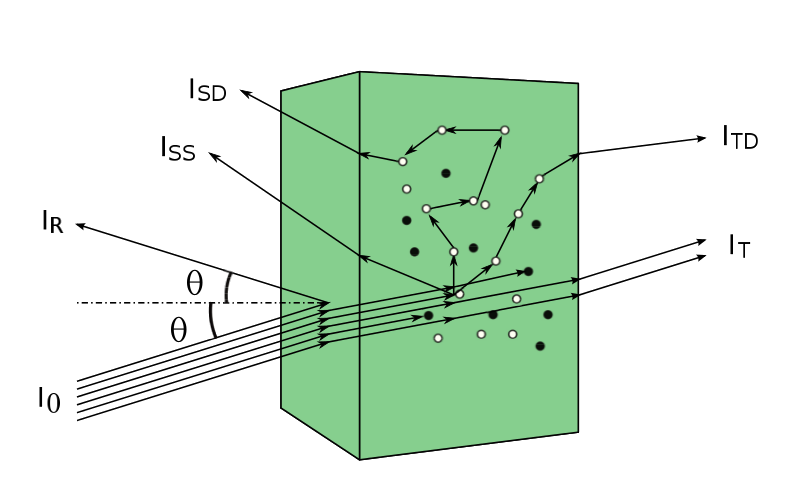
\includegraphics[scale = 0.50]{graphic/light_interaction.png}}
	\caption{Interakcja promieniowania elektromagnetycznego z~materią. Natężenie wejściowe światła~($I_{0}$), odbite~($I_{R}$), 
	rozproszone wstecz ($I_{SS}$, $I_{SD}$), wyjściowe ($I_{TD}$, $I_{T}$)}
	~\\	
	(źródło: Na podstawie \cite{Valisue:Thesis:2011})
	\label{rys:light_interaction}
\end{figure}
Zmiana kierunku rozchodzenia się fali na granicy dwóch ośrodków, powodująca, że pozostaje ona w~ośrodku, w~którym się rozchodzi definiuje prawo 
odbicia~\cite{Feyn:2012}. Kąt odbicia jest równy kątowi padania, a~promień padający, promień odbity i~normalna do powierzchni odbicia leżą w~jednej 
płaszczyźnie~(rys.~\ref{rys:refraction}). W~wyniku odbicia zmienia się tylko kierunek rozchodzenia się fali, nie zmienia się jej długość.

\begin{figure}[ht]
	\centerline{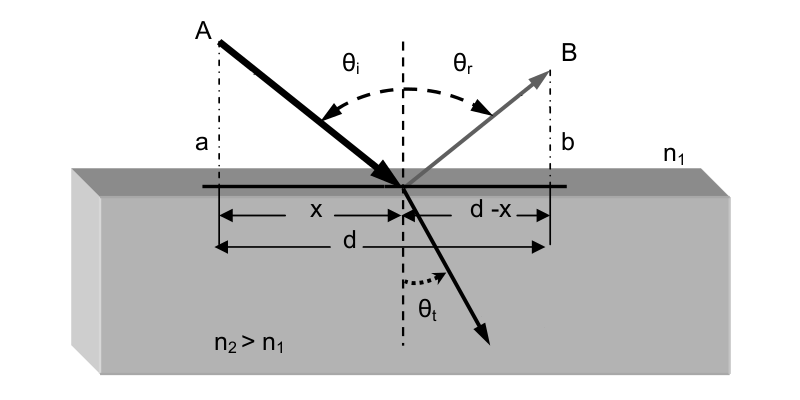
\includegraphics[scale = 0.53]{graphic/refraction.png}}
	\caption{Załamanie i~odbicie promieniowania elektromagnetycznego na granicy dwóch ośrodków o~współczynnikach refrakcji $n_{1}$~i~$n_{2}$}
	~\\
	(źródło: Na podstawie \cite{Yavari:PhD:2006})
	\label{rys:refraction}
\end{figure}


\section{Absorpcja}
\label{sec:Absorpcja}
%---------------------------------------------------------------------------

Natężenie wiązki promieniowania elektromagnetycznego jest redukowane w~miarę przenikania przez ośrodek materialny na skutek 
oddziaływania z~materią. Pochłonięta część energii promieniowania pierwotnego przechodzi przy tym w~inne formy energii (energia wewnętrzna ośrodka, 
energia wzbudzenia lub jonizacji, energia wtórnego promieniowania elektromagnetycznego)~\cite{Feyn:2012}.

Z~mikroskopowego punktu widzenia oraz według zasad fizyki kwantowej, poziomy energetyczne atomów i~cząsteczek są skwantyzowane~\cite{Yavari:PhD:2006}.
W~procesie absorpcji światło zachowuje się jak strumień cząstek elementarnych i~może być pochłaniane tylko w~określonych porcjach energii $E$, których 
wielkość zależy od częstotliwości $\nu$~(\ref{equ:planc}):

\begin{equation}
	E = h\nu
\label{equ:planc}
\end{equation}
$h$ - stała Plancka.\\

Kwant światła, czyli foton niosący określoną porcję energii może oddziaływać z~elektronem walencyjnym w~atomie substancji ośrodka. Jeżeli 
energia fotonu równa jest różnicy energii pomiędzy dowolnym stanem wzbudzonym elektronu a~stanem podstawowym, wówczas foton zostanie pochłonięty 
(rys.~\ref{rys:absorption}). 
Gdy energia fotonu jest inna, wówczas albo przechodzi on przez substancję bez przeszkód, albo jest rozpraszany. Na skutek absorpcji fotonu elektron 
przechodzi w~stan wzbudzenia o~wyższej energii~\cite{Yavari:PhD:2006}.

\begin{figure}[ht]
	\centerline{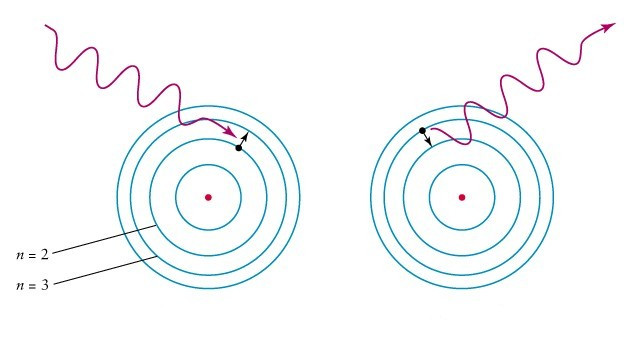
\includegraphics[scale = 0.62]{graphic/absorption.jpg}}
	\caption{Absorpcja spontaniczna. Elektron pochłania energię fotonu, dzięki czemu następuje wzbudzenie go na wyższy poziom energetyczny. Emisja 
	 	 to zjawisko odwrotne do absorpcji}
	~\\
	(źródło: http://www.candela.strefa.pl) 
	\label{rys:absorption}
\end{figure}

\subsection{Prawo Lamberta-Bouguera}
\label{subsec:LambertBouguer}
%---------------------------------------------------------------------------
Prawo Lamberta-Bouguera ilościowo opisuje proces absorpcji światła przez roztwory substancji barwnych podczas przenikania promieniowania 
monochromatycznego przez roztwór. Zależność opisująca stopień pochłaniania promieniowania w~stosunku do grubości ośrodka absorbującego po raz 
pierwszy podana została przez Bouguera w~1729 roku w~następującej postaci~\cite{Yavari:PhD:2006}:

\begin{equation}
	\frac{dI}{I} = \mu_{a}(\lambda)dx
	\label{equ:LambertBouguer}
\end{equation}
gdzie:\\
$x$ - grubość warstwy ośrodka,\\
$I$ - natężenie światła padającego,\\
$\mu_{a}(\lambda)$ - współczynnik absorpcji światła.\\\\
Rozwiązanie równania~(\ref{equ:LambertBouguer}) względem $x$ pokazuje, iż wartość promieniowania przenikającego przez roztwór maleje wykładniczo 
wraz z~grubością ośrodka~(rys.~\ref{rys:bouguer}). W~odlegości $x$ od powierzchni nadawczej w~ośrodku o~współczynniku pochłaniania $\mu_{a}(\lambda)$ wynosi:

\begin{equation}
	I(x) = Ie^{-\mu_{a}(\lambda) x}
\end{equation}
gdzie:\\
$I(x)$ - natężenie światła po przejściu przez warstwę ośrodka o~grubości~$x$\\
$e$ - podstawa logarytmu naturalnego.\\

\begin{figure}[ht]
	\centerline{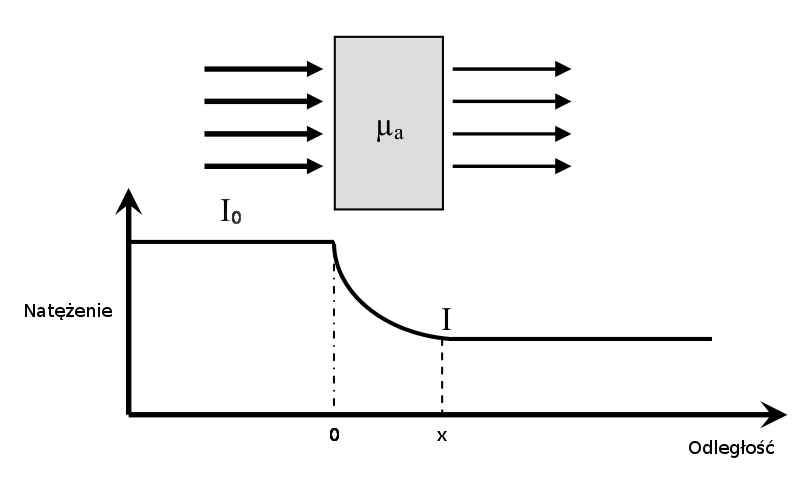
\includegraphics[scale = 0.5]{graphic/bouguer.png}}
	\caption{Absorpcja promieniowania w~jednorodnym ośrodku pochłaniającym o~współczynniku absorpcji $\mu_{a}$}
	~\\
	(źródło: Na podstawie \cite{Yavari:PhD:2006})
	\label{rys:bouguer}
\end{figure}

\subsection{Prawo Lamberta-Beera}
\label{subsec:BeerLambert}

W~1852 roku na bazie prowadzonych doświadczeń dowiedziono, iż wartość współczynnika absorpcji $\mu_{a}(\lambda)$ dla określonej długości fali jest wprost 
proporcjonalna do stężenia substancji absorbującej~\cite{Yavari:PhD:2006}.\\

\begin{equation}
	\mu_{a}(\lambda) = c\alpha(\lambda)
\end{equation}
gdzie:\\
$c$ - stężenie molowe substancji absorbującej w~roztworze,\\
$\alpha(\lambda)$ - molowy współczynnik absorpcji zwany absorbancją molową.

\noindent Zestawiając prawo Lamberta-Bouguera z~prawem Lamberta-Beera otrzymano kompletny opis zjawiska absorpcji promieniowania w~ośrodku absorbującym w~postaci:

\begin{equation}
	I(x) = Ie^{(-c\alpha(\lambda) x)}\\
\end{equation}
 
\begin{figure}[ht]
	\centerline{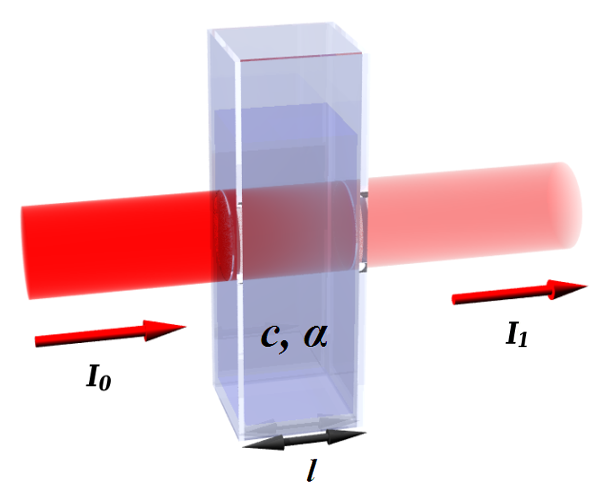
\includegraphics[scale = 0.44]{graphic/Beer_lambert.png}}
	\caption{Absorpcja światła przechodzącego przez substancję o~stężeniu molowym $c$ i~molowym współczynniku absorpcji $\alpha(\lambda)$}
	~\\
	(źródło: http://pl.wikipedia.org)
	\label{rys:Beer_lambert}
\end{figure}


\subsubsection{Prawo addytywności absorpcji}
\label{subsub:add}

W~przypadku roztworów złożonych z~wielu substancji o~różnych właściwościach optycznych, matematyczna reprezentacja prawa Lamberta-Beera jest superpozycją 
absorpcji każdego składnika z~osobna~\cite{Yavari:PhD:2006}:  
\begin{equation}
	I(x) = Ie^{-A}
	\label{equ:multilayer1}
\end{equation}
Dla środowiska niejednorodnego~(rys.~\ref{rys:multilayer}) absorbancja $A$ określana jest według zależności:
\begin{equation}
	A=c_{1}\alpha_{1}(\lambda)x_{1} + c_{2}\alpha_{2}(\lambda)x_{2} + ... + c_{i}\alpha_{i}(\lambda)x_{i} = \sum_{i=1}^{n}c_{i}\alpha_{i}(\lambda)x_{i}\\
	\label{equ:multilayer2}
\end{equation}
\begin{figure}[!ht]
	\centerline{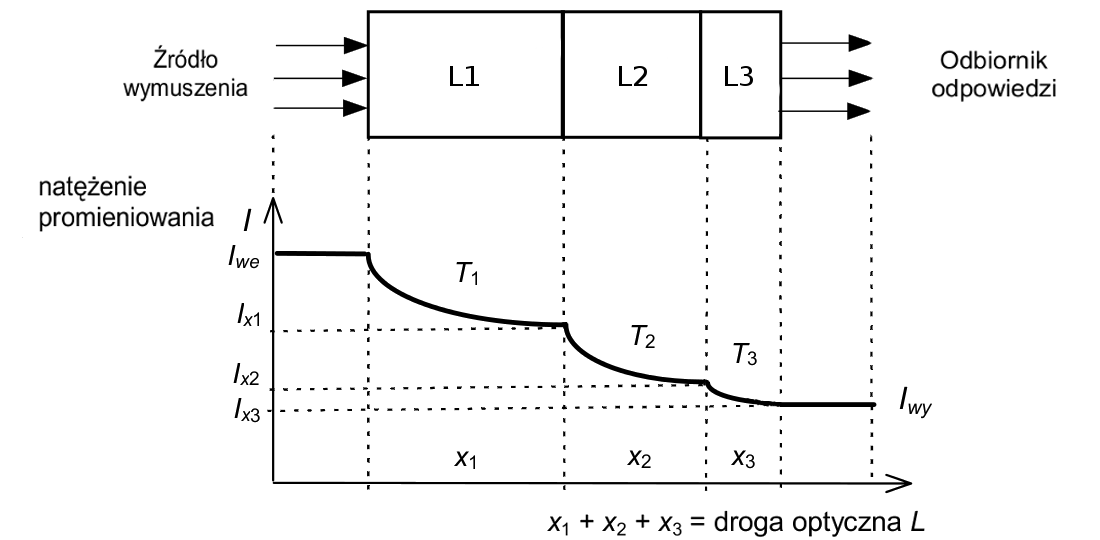
\includegraphics[scale = 0.40]{graphic/multilayer.png}}
	\caption{Absorpcja promieniowania przechodzącego przez ośrodek złożony}
	~\\
	(źródło: Na podstawie \cite{Cys:2007})
	\label{rys:multilayer}
\end{figure}\\

\noindent W~przypadku ośrodka homogenicznego dla $i$ różnych substancji o~odmiennych właściwościach optycznych całkowita absorbancja wynosi:
\begin{equation}
	A=(c_{1}\alpha_{1}(\lambda) + c_{2}\alpha_{2}(\lambda) + ... + c_{i}\alpha_{i}(\lambda))x = (\sum_{i=1}^{n}c_{i}\alpha_{i}(\lambda))x\\
	\label{equ:multilayer3}
\end{equation}
Korzystając z~równania~(\ref{equ:multilayer1}) i~(\ref{equ:multilayer3}), prawo Lamberta-Beera pozwala określić stężenia $n$ różnych substancji absorbujących 
w~homogenicznym środowisku, jeśli absorpcja światła jest mierzona dla $n$ różnych długości fali przy znanych współczynnikach absorbancji molowej 
$\alpha_{i}(\lambda)$~\cite{Katja:2011}.

\section{Rozpraszanie}
\label{sec:Rozpraszanie}
%---------------------------------------------------------------------------

Nazwą tą określa się zjawisko oddziaływania światła z~materią, w~wyniku którego następuje zmiana kierunku rozchodzenia się promieniowania, z~wyjątkiem zjawisk opisanych 
przez odbicie i~załamanie. Rozpraszanie wywołuje złudzenie świecenia ośrodka pod wpływem oddziaływania z~promieniowaniem elektromagnetycznym z~zakresu fal widzialnych~(rys.~\ref{rys:scattering}). 
\begin{figure}[ht]
	\centerline{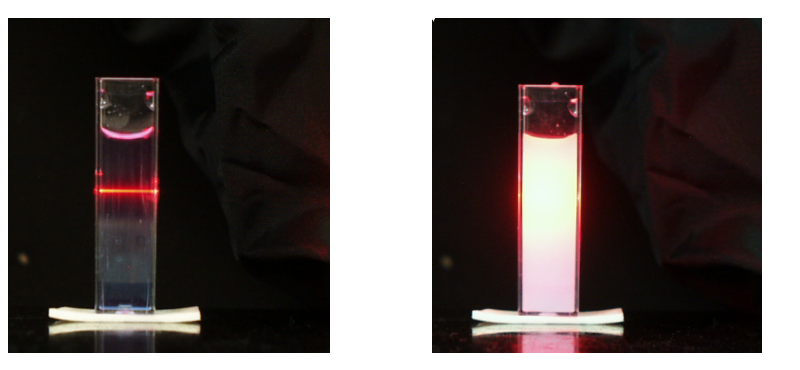
\includegraphics[scale = 0.45]{graphic/scattering.png}}
	\caption{Interakcja promieniowania świetlnego z~materią w~ośrodku nierozpraszającym i~rozpraszającym}
	~\\
	(źródło: Na podstawie \cite{Dwyer:2008})
	\label{rys:scattering}
\end{figure}

\noindent Rozróżnia się następujące jego rodzaje~\cite{Zee:1992}:
\begin{itemize}
	\item sprężyste – podczas rozpraszania nie następuje zmiana energii światła,
	\item niesprężyste – następuje zmiana energii promieniowania w~wyniku rozproszenia.
\end{itemize}

Zjawisko rozpraszania światła można podzielić na trzy rodzaje interakcji światło-cząstka: rozpraszanie Rayleigha, rozpraszanie Mie oraz rozpraszanie Ramana~\cite{Nui:2007}. 
Zjawisko Rayleigha zachodzi przy długości fali $\lambda$ znacznie większej niż wymiary cząstek ośrodka, gdzie rozpraszanie Mie 
występuje przy wymiarach porównywalnych. Zarówno rozpraszanie Rayleigha, jak i~rozpraszanie Mie są sprężyste i~powodują zmianę tylko trajektorii rozproszonego 
fotonu. Teoria Ramana natomiast opisuje zjawisko, w~którym trajektoria rozproszonego fotonu ulega zmianie, ale dodatkowo powoduje emisję światła, zwykle o~większej 
długości fali~\cite{Nui:2007}.

\subsection{Zmodyfikowane prawo Lamberta-Beera dla rozpraszania}
\label{subsec:LBrozpraszanie} 

Poprzez analogię do zjawiska absorpcji promieniowania, efekt rozpraszania fotonów wewnątrz medium transmisyjnego również wprowadza osłabienie wiązki w~kierunku 
propagacji fali elektromagnetycznej. Współczynnik $\mu_{s}$ opisuje stratę natężenia promieniowania na skutek rozproszenia, co wspólnie ze zjawiskiem absorpcji 
zapisuje się następująco:

\begin{equation}
	I(x) = Ie^{-\mu_{t}x}
\end{equation}
dla
\begin{equation}
	\mu_{t} = \mu_{a} + \mu_{s}
\end{equation}
gdzie:\\
$\mu_{a}$ - współczynnik absorpcji promieniowania,\\
$\mu_{s}$ - współczynnik rozpraszania promieniowania.\\

W~tkankach biologicznych dominujący wpływ mają zjawiska opisane przez Rayleigha oraz Mie~\cite{Nui:2007}, których podstawową różnicą jest odmienna kierunkowość 
natężenia promieniowania wtórnego~(rys.~\ref{rys:scattering_3}). Rozkład kątowy intensywności światła rozproszonego dla zjawiska Rayleigha jest osiowo symetryczny 
względem linii przechodzącej przez elementarną cząstkę rozpraszającą w~kierunku propagacji fali padającej. Maksymalne rozpraszanie występuje w~płaszczyźnie równoległej 
do kierunku wiązki padającej~(rys.~\ref{rys:scattering_3}a). Rozpraszanie Mie charakteryzuje silna zależność rozkładu intensywności od kierunku. Obserwuje się asymetrię 
między rozpraszaniem w~przód i~w~tył: przeważa rozpraszanie w~przód~(rys.~\ref{rys:scattering_3}b).
\begin{figure}[!ht]
	\centerline{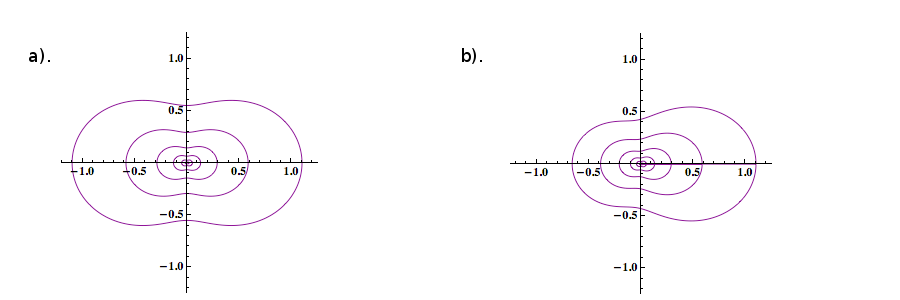
\includegraphics[scale = 0.62]{graphic/scattering_3.png}}
	\caption{Zależność rozkładu intensywności promieniowania rozproszonego od kierunku propagacji dla zjawiska Rayleigha~(a) oraz Mie~(b)}
	~\\
	(źródło: http://pages.vassar.edu)
	\label{rys:scattering_3}
\end{figure}

\subsection{Funkcja fazowa i~współczynnik anizotropii}
\label{subsec:PhaseAnisotropy}

Rozpraszanie promieniowania w~tkankach nie jest zjawiskiem izotropowym~\cite{Yavari:PhD:2006}. Natężenie promieniowania emitowanego jest zmienne w~zależności 
od kąta odchylenia od kierunku propagacji.

Należy zdefiniować funkcję fazową $p(\theta)$ wyznaczającą prawdopodobieństwo $p$ rozproszenia kwantu promieniowania pod danym kątem $\theta$. Prawdopodobieństwo 
rozproszenia fotonu zależy wyłącznie od wyboru kąta odchylenia pomiędzy wektorem jednostkowym rozproszenia $\hat{s}'$ a~wektorem zgodnym z~kierunkiem propagacji fali 
padającej $\hat{s}$:
\begin{equation}
	p(\theta)=p(\hat{s}', \hat{s})
\end{equation}
Funkcja fazowa $p(\theta)$ Henyeya-Greensteina~(\ref{equ:HenyeyGreenstein}) jest stosowana podczas analizy zjawiska rozpraszania w~ośrodkach złożonych z~tkanek 
biologicznych~\cite{Yavari:PhD:2006}. 

\begin{equation}
	p(\theta)=\frac{1}{4\pi}\frac{1-g^2}{(1+g^2-2gcos(\theta))^{\frac{3}{2}}}
	\label{equ:HenyeyGreenstein}
\end{equation}
gdzie spełniona jest zależność:

\begin{equation}
	\int_{0}^{\pi} p(\theta)2\pi sin(\theta)d\theta=1
\end{equation}
Parametr $g$ opisuje stopień anizotropii rozpraszania promieniowania w~ośrodku.
Wpływ współczynnika anizotropii na charakterystykę kierunkową rozpraszania przedstawiono na rysunku \ref{rys:anisotropy}. Zakres 
wartości parametru $g$~zawiera się w~zakresie od -1~(całkowite rozpraszanie w~tył) do wartości 1~(całkowite rozpraszanie w~przód).
Dla $g=0$ rozpraszanie ma charakter izotropowy. 

\subsection{Zredukowany współczynnik rozpraszania}
\label{subsec:ReducedFactor}

Wyrażenie na współczynnik efektywnego rozpraszania w~ośrodku rozpraszającym powinno uwzględniać zarówno współczynnik rozpraszania $\mu_{s}$,
jak i~współczynnik anizotropii~$g$. 
\noindent Zredukowany współczynnik rozpraszania $\mu_{s}'$ łączy wspomniane parametry w~następujący sposób:
\begin{equation}
	\mu_{s}'=\mu_{s}(1-g)
	\label{equ:reduced_mu}
\end{equation}
\begin{figure}[ht]
	\centerline{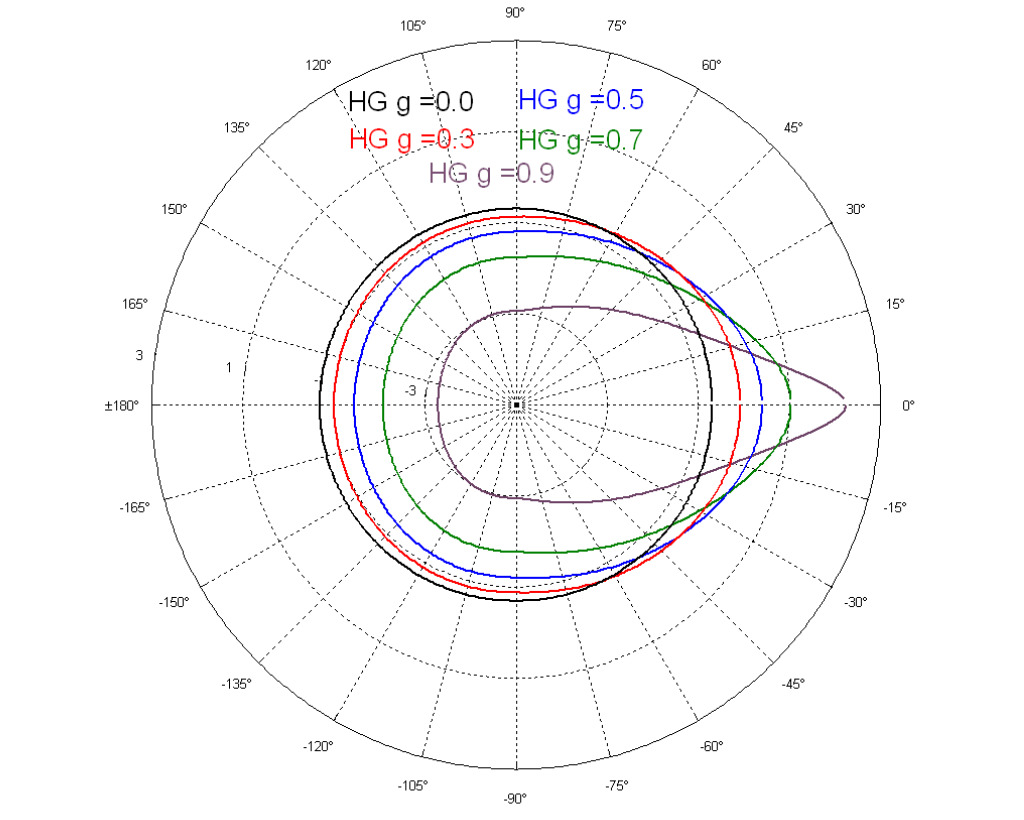
\includegraphics[scale = 0.45]{graphic/HenyeyGreenstein.png}}
	\caption{Przebieg funkcji Henyeya-Greensteina dla wybranych wartości współczynnika anizotropii $g$}
	~\\
	(źródło: http://openi.nlm.nih.gov)
	\label{rys:anisotropy}
\end{figure}

\noindent Całkowity współczynnik tłumienia promieniowania wewnątrz ośrodka rozpraszającego i~absorbującego po uwzględnieniu współczynnika anizotropii przedstawia
się następująco:
\begin{equation}
	\mu_{t}'=\mu_{a} + \mu_{s}'
\end{equation}


\renewcommand{\figurename}{Rys.}

\chapter{Metodyka pomiaru wysycenia krwi i~częstości akcji serca}
\label{cha:Metodyka}

\fontsize{14}{15}\selectfont
%---------------------------------------------------------------------------

Pulsoksymetria to nowoczesna, nieinwazyjna i~bezbolesna metoda badania tętna i~utlenowania krwi. Oparta na elementarnych prawach fizyki, pozwala 
uzyskać cenne informacje o~układzie krążenia, a~dokładniej - jego zdolności do transportu tlenu w~organizmie. Metoda polega na zasadzie spektrofotometrycznego 
pomiaru wysycenia tlenem hemoglobiny, gdyż hemoglobina utlenowana i~odtlenowana wykazują odmienne właściwości optyczne. Jednocześnie rejestrowana jest również 
częstotliwość pracy serca (tętno).

 
\section{Rola krwi w~procesie wymiany gazowej}
\label{sec:RolaKrwi}

Wymiana gazowa to proces, podczas którego dochodzi do dyfuzji gazów i~ich wymiany między organizmem a~otoczeniem przy pomocy krwi. 
U~człowieka układ krwionośny jest zamknięty~\cite{Fizj:2007}. Znaczy to, że krew nieustannie obiega organizm w~całym systemie połączonych ze sobą 
naczyń krwionośnych. Pompą wymuszającą ten obieg jest serce. Krążenie krwi odbywa się na dwóch drogach: obwodowej oraz płucnej~(rys.~\ref{rys:circ}).

Wymiana gazowa następuje pomiędzy dwoma składnikami atmosfery: tlenem i~dwutlenkiem węgla. W~płucach z~powodu wyższego ciśnienia parcjalnego tlenu 
w~pęcherzykach następuje utlenowanie krwi w~małym obiegu krwi i~dostarczanie jej do tkanek obwodowych.
 
Dostarczany tlen jest niezbędny do zwiększenia wydajności spalania glukozy oraz do tego, by potencjalna energia związków organicznych pochodzących 
z~pokarmu została z~możliwie największą wydajnością zużyta we wszystkich procesach życiowych~\cite{Fizj:2007}.

\begin{figure}[ht]
	\centerline{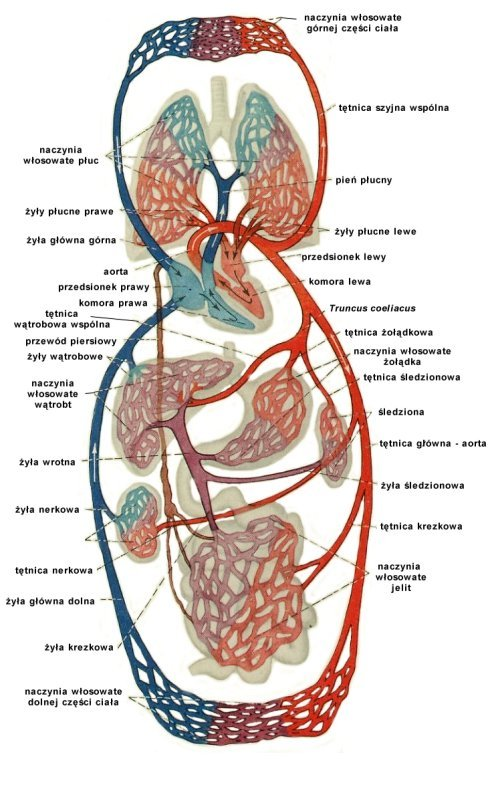
\includegraphics[scale = 0.84]{graphic/obieg_krwi.jpg}}
	\caption{Duży i~mały obieg krwi}
	~\\
	(źródło: http://anatomiac.w.interia.pl)
	\label{rys:circ}
\end{figure}
Krew w~obiegu obwodowym wymienia tlen na dwutlenek węgla w~tkankach organizmu. W~miejscu docelowym krew, poprzez ściany naczyń włosowatych, oddaje tlen 
tkankom o~niższym jego ciśnieniu parcjalnym. Krew częściowo również transportuje dwutlenek węgla~($CO_{2}$), jednak ten jest przenoszony głównie przez 
osocze w~postaci jonowej ($HCO_{3}$)~\cite{Fizj:2007}.
 
\subsection{Skład i~funkcje krwi}
\label{subsec:SkladKrwi}

Krew jest rodzajem tkanki łącznej płynnej. Składa się z~osocza oraz elementów morfotycznych~\cite{Fizj:2007}, których zawartość przedstawia 
tabela~(tab.~\ref{tab:Morfotyczne}).\\

\begin{table}[h]\large
	\caption{Wartości prawidłowe składników morfotycznych i~chemicznych we krwi~\cite{SzGa11}}
	\label{tab:Morfotyczne}
	\begin{center}
	\begin{tabular}{|c||c|c|}
	\hline
	Składnik & \multicolumn{2}{|c|}{Normy}	\\
	\hline \hline

	\multirow{2}{*}{Erytrocyty (RBC)} & \multicolumn{2}{|c|}{$4,2 - 5,4~ mln/mm^3$ (M)} \\
	\cline{2-3} & \multicolumn{2}{|c|}{$3,4 - 5,2~mln/mm^3$ (K)} \\ 
	\hline	

	Leukocyty (WBC) & \multicolumn{2}{|c|}{$4 - 7~tys/mm^3$} \\
	\hline

	Trombocyty (PLT) & \multicolumn{2}{|c|}{$150 - 300~tys/mm^3$} \\
	\hline
	\multirow{2}{*}{Hematokryt (HC)} & \multicolumn{2}{|c|}{$42\% - 52\%$ (M)} \\
	\cline{2-3} & \multicolumn{2}{|c|}{$37\% - 47\%$ (K)} \\
	\hline

	MCHC  & \multicolumn{2}{|c|}{$32 - 36~g/100 ml$}\\
	\hline
	\multirow{2}{*}{Hemoglobina} & \multicolumn{2}{|c|}{$14 - 18~g/dl$ (M)} \\ 
	\cline{2-3} & \multicolumn{2}{|c|}{$12 - 16~g/dl$ (K)} \\ 
	\hline

	Karboksyhemoglobina & \multicolumn{2}{|c|}{do 3\% hemoglobiny} \\
	\hline
	\end{tabular}
	\end{center}
	~\\
	(źródło: Na podstawie \cite{SzGa11})
\end{table}
Osocze krwi stanowi płynną część krwi, stanowiącą 4,5\% ciężaru ciała, w~której zawieszone są elementy morfotyczne~(rys.~\ref{rys:osocze}).
Składa się głównie z~wody (92\%) i~rozpuszczonych w~niej białek osocza: albumin, globulin, fibrynogenu i~innych czynników krzepnięcia (zarówno aktywujących, jak 
i~hamujących ten proces), ciał tłuszczowych, glukozy, elektrolitów i~wielu innych składników organicznych i~nieorganicznych~\cite{Fizj:2007}.

\begin{figure}[!ht]
	\centerline{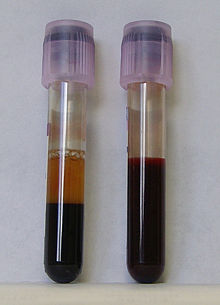
\includegraphics[scale = 0.64]{graphic/osocze.jpg}}
	\caption{Próbki krwi. Po prawej krew świeżo pobrana, po lewej krew z~substancją zapobiegającą krzepnięciu. Widoczne jaśniejsze osocze, pod 
		 którym osadziły się składniki komórkowe}
	~\\
	(źródło: Na podstawie \cite{Dwyer:2008})
	\label{rys:osocze}
\end{figure}
\noindent Transport atomów tlenu przez krew w~ustroju jest możliwa dzięki cząsteczkom hemoglobiny zawartej w~krwinkach czerwonych. 
Hemoglobina ($Hb$) jest białkiem, składającym się z~czterech łańcuchów polipeptydowych~\cite{Fizj:2007}, z~których każdy łączy się w~płucach 
z~jedną cząsteczką~$0_{2}$~(rys.~\ref{rys:hemoglobina}). 
\begin{figure}[!ht]
\centerline{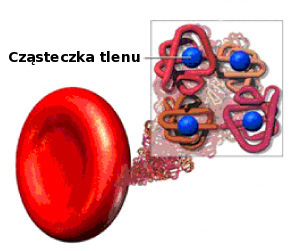
\includegraphics[scale = 0.66]{graphic/hemoglobina.jpg}}
	\caption{Cząsteczki hemoglobiny zawarte w~erytrocytach umożliwiają wiązanie oraz transport cząsteczek tlenu}
	\label{rys:hemoglobina}
	~\\
	(źródło: Na podstawie \cite{Dwyer:2008})
\end{figure}

\noindent Nietrwałe połączenie cząsteczek tlenu z~cząsteczką hemoglobiny tworzy oksyhemoglobinę~($HbO_{2}$).

\subsection{Saturacja $SaO_{2}$ a~$SpO_{2}$}
\label{subsec:Saturacja}

Hemoglobina ($Hb$) wykazuje zdolność do wiązania z~wieloma pierwiastkami oraz związkami chemicznymi tworząc trwałe lub nietrwałe połączenia. 
Oksyhemoglobina ($HbO_{2}$), karboksyhemoglobina ($HbCO$), sulfohemoglobina ($SulfHb$) oraz methemoglobina ($MetHb$) to najistotniejsze związki 
z~punktu widzenia efektywności transportu tlenu. 

W~diagnostyce medycznej rozróżnia się dwa wskaźniki wysycenia krwi: $SpO_{2}$ oraz $SaO_{2}$. 
Parametr $SaO_{2}$ definiowany jako procentowa zawartość oksyhemoglobiny w~całkowitej ilości hemoglobiny~(\ref{equ:SaO2}), 
wyznaczany jest metodą inwazyjną opartą o~analizę chemiczną pobranej próbki krwi~(in~vitro).

\begin{equation}
\label{equ:SaO2}
	SaO_{2} = \frac{HbO_{2}}{HbO_{2} + Hb + HbCO + metHb + SulfHb} * 100\%
\end{equation}

Inwazyjna metoda wyznaczania saturacji $SaO_{2}$ pozwala na określenie poprawnej zawartości hemoglobiny utlenowanej, bez uwzględnienia hemoglobiny 
dysfunkcyjnej. Istnienie wielu rodzajów dyshemoglobiny niezdolnej do prawidłowego transportu tlenu, jak $metHb$ oraz $HbCO$ wprowadza błędy pomiarowe
nasycenia krwi przy pomiarach metodami optycznymi. Metody pomiaru saturacji częściowej $SpO_{2}$ oparte o~analizę stopnia absorpcji promieniowania 
przez składniki krwi nie odróżniają odmian hemoglobiny połączonej ze związkami tlenu~\cite{Fizj:2007}. Skutkiem niedoskonałości metod optycznych jest
zawyżanie wartości nasycenia w~przypadku występowania hemoglobiny dysfunkcyjnej~(\ref{equ:SpO2}). 

\begin{equation}
\label{equ:SpO2}
	SpO_{2} = \frac{HbO_{2} + HbCO + metHb}{HbO_{2} + Hb + HbCO + metHb + SulfHb} * 100\%
\end{equation}
\\
\noindent Podczas zatrucia tlenkiem węgla, którego powinowactwo do hemoglobiny jest 250-300 razy większe niż tlenu, wskaźnik nasycenia $SpO_{2}$ 
osiąga wartość 100\%, mimo braku zdolności do prawidłowego transportu tlenu. 

\section{Spektrofotometria 'in vivo'}
\label{sec:InVivo}

Spektroskopia absorpcyjna i~odbiciowa w~bliskim nadfiolecie, świetle widzialnym oraz w~podczerwieni znajdują szerokie zastosowanie w~chemii analitycznej, 
biologii, medycynie i~badaniach materiałowych.
Selektywna absorpcja zespołów komórek umożliwia wykorzystanie w~diagnostyce medycznej zasad i~praw spektrofotometrii. Zdecydowana większość analiz 
medycznych przeprowadzanych jest przy wykorzystaniu zasad fotometrii, a~z~tego aż około 90\% opiera się na zasadach spektrofotometrii. Oznacza 
się w~ten sposób poziom hormonów, przeprowadza testy enzymatyczne, bada kinetykę reakcji chemicznych~\cite{Cys:2007}. 

Badania spektofotometryczne przeprowadzane są w~układzie łącza optycznego: źródło promieniowania, kuweta pomiarowa, odbiornik promieniowania.
Spektrofotometria 'in vivo' jest badaniem laboratoryjnym przeprowadzanym na organizmie żywym bez konieczności pozyskiwania próbek metodami inwazyjnymi.

\subsection{Okno optyczne tkanek}
\label{subsec:OknoOptyczne}

Badany obiekt biologiczny~(rys.~\ref{rys:finger}) składa się z~ciał stałych, cieczy i~gazów absorbujących promieniowanie świetlne, 
charakteryzujących się indywidualnym widmem absorpcyjnym~\cite{Nui:2007}. Woda, związki hemoglobiny, lipidy, melanina, mioglobina, 
cytochromy, bilirubina oraz karotenoidy to podstawowe chromofory ustroju~\cite{Haggblad:2008}. 

\begin{figure}[ht]
\centerline{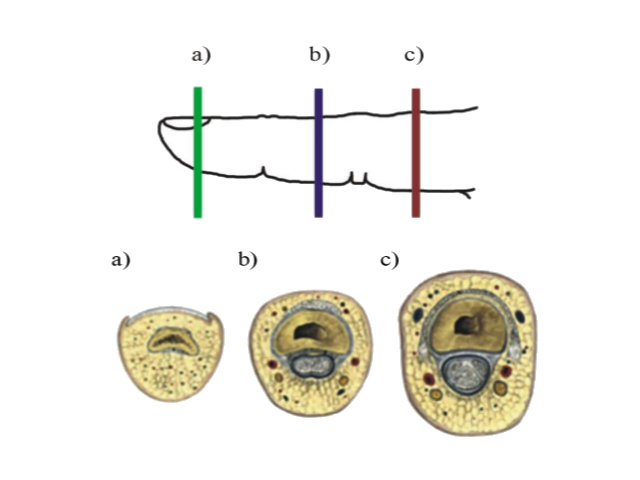
\includegraphics[scale = 0.56]{graphic/finger.png}}
	\caption{Kolejne przekroje tkanek palca ludzkiego}
	\label{rys:finger}
	~\\
	(źródło: Na podstawie \cite{Cys:2007})
\end{figure}

Równanie~(\ref{equ:multilayer2}) przedstawia całkowity współczynnik absorpcji niejednorodnej mieszaniny związków, który jest równy sumie ich indywidualnych 
współczynników pochłaniania.

Celem zwiększenia skuteczności pomiaru absorpcji użytecznego promieniowania świetlnego przez składniki krwi, należy zminimalizować wpływ pochłaniania użytecznego
promieniowania przez pozostałe chromofory środka. Odmienne widma absorpcyjne związków pochłaniających zmuszają do obrania optymalnego zakresu promieniowania
świetlnego.

\subsubsection{Woda}
\label{subsubsec:Woda}

Woda stanowi od 60\% do 80\% całkowitej masy ciała i~jest głównym składnikiem płynów ustroju, m.in.~krwi i~limfy. Z~powodu wysokiej koncentracji, $H_{2}O$ 
w~większości tkanek biologicznych jest najistotniejszym medium absorbującym w~pomiarach spektroskopowych. Widmo absorpcyjne wody w~zakresie 200~-~10000~nm 
oraz 650~-~1050~nm przedstawia rysunek \ref{rys:water}.

\begin{figure}[ht]
\centerline{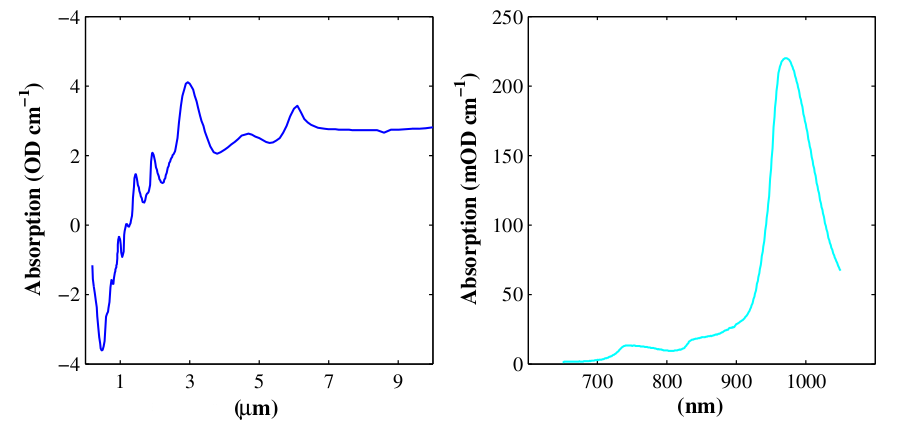
\includegraphics[scale = 0.56]{graphic/water.png}}
	\caption{Widmo absorpcyjne czystej wody}
	\label{rys:water}
	~\\
	(źródło: Na podstawie \cite{Haggblad:2008})
\end{figure}
\noindent W~obszarze 200~-~900 nm istnieje przedział stosunkowo niskiej absorpcji promieniowania. Powyżej granicy 900 nm współczynnik pochłaniania gwałtownie 
wzrasta, skutecznie pochłaniając promieniowanie z~tego zakresu długości fali.

\subsubsection{Związki hemoglobiny}
\label{subsubsec:hemoglobina}

Zdolność hemoglobiny do absorpcji promieniowania świetlnego silnie zależy od zawartości tlenu. Hemoglobina bogata w~cząsteczki $O_{2}$ (oksyhemoglobina) 
wykazuje lokalne maksima pochłaniania dla długości fali w~zakresie 576~-~542 nm oraz globalne maksimum dla 415~nm. Widmo absorpcyjne deoksyhemoglobiny 
posiada lokalne maksima pochłaniania dla 420~nm, 555~nm oraz 756~nm~(rys.~\ref{rys:hb}). Dla promieniowania o~długości fali do 560~nm współczynniki absorpcji 
oksyhemoglobiny oraz deoksyhemoglobiny są zbliżone.  
\begin{figure}[!ht]
\centerline{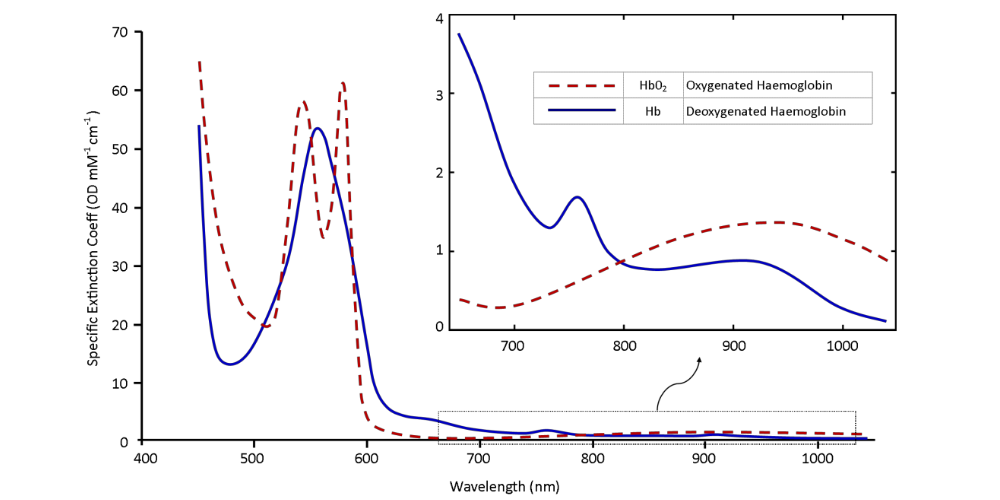
\includegraphics[scale = 0.54]{graphic/hb.png}}
	\caption{Widmo absorpcyjne deoksyhemoglobiny i~oksyhemoglobiny. Charakterystyczny punkt izozbestyczny dla 800 nm}
	\label{rys:hb}
	~\\
	(źródło: Na podstawie \cite{Haggblad:2008})
\end{figure}

\noindent Istotnym obszarem z~punktu widzenia spektrofotometrii jest zakres promieniowania od 600~nm do 1000~nm, gdzie związki hemoglobiny wykazują odrębne właściwości 
optyczne~(rys.~\ref{rys:blood}). Dla długości fali około 800~nm istnieje punkt izozbestyczny, w~którym absorpcja dla obu rodzajów hemoglobiny jest identyczna.
\subsubsection{Mioglobina}
\label{subsubsec:hemoglobina}

Jest to białko zbliżone budową do hemoglobiny, służące do magazynowania tlenu w~mięśniach czerwonych (poprzecznie prążkowanych)~\cite{Haggblad:2008}. 
Wyróżnia się deoksymioglobinę, oksymioglobinę, karboksymioglobinę oraz metmioglobinę. Rysunek~\ref{rys:mioglobin} przedstawia widmo absorpcyjne 
związków mioglobiny.
\begin{figure}[h]
\centerline{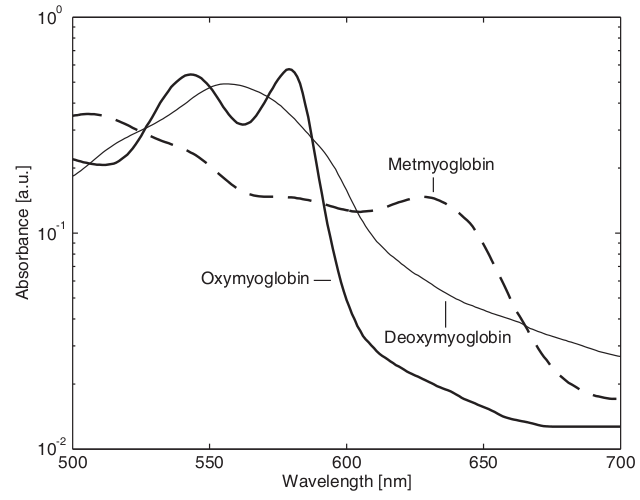
\includegraphics[scale = 0.50]{graphic/mioglobin.png}}
	\caption{Widmo absorpcyjne deoksymioglobiny, oksymioglobiny oraz metmioglobiny}
	\label{rys:mioglobin}
	~\\
	(źródło: Na podstawie \cite{Haggblad:2008})
\end{figure}

\subsubsection{Melanina}
\label{subsubsec:melanina}

Melanina to pigment występujący w~skórze właściwej, naskórku, włosach oraz w~tęczówce oka, odpowiedzialny za ich barwę. Melaniny w~skórze chronią jej 
głębsze warstwy przed szkodliwym promieniowaniem ultrafioletowym UV zawartym w~promieniowaniu słonecznym. Pod wpływem promieni słonecznych ilość melaniny 
zwiększa się, powodując przejściową zmianę zabarwienia skóry~\cite{Haggblad:2008}. Wśród melanin wyróżnia się m.in. eumelaninę, feomelaninę i~neuromelaninę. 
Eumelanina jest barwnikiem czarnobrązowym, feomelanina jest pigmentem o~zabarwieniu żółtoczerwonym.
\begin{figure}[h]
\centerline{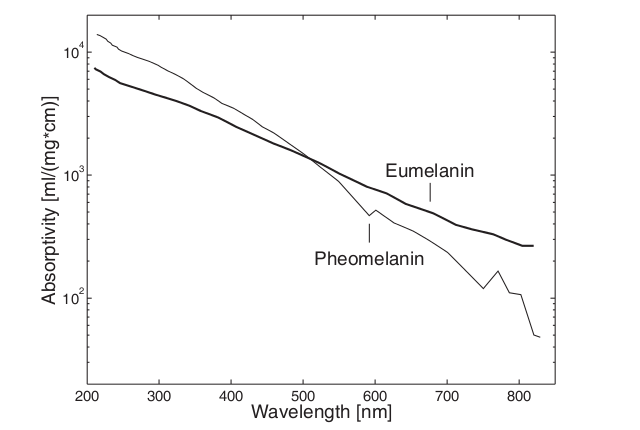
\includegraphics[scale = 0.55]{graphic/melanin.png}}
	\caption{Widmo absorpcyjne eumelaniny oraz feomelaniny}
	\label{rys:melanin}
	~\\
	(źródło: Na podstawie \cite{Haggblad:2008})
\end{figure}

\subsubsection{Inne chromofory}
\label{subsubsec:hromofory}

Łączna ilość endogennych związków absorbujących, znajdujących się w~tkankach żywych jest ogromna. Jednak większość z~nich jest obecnych tylko
w~mniejszych stężeniach, co czyni je mniej znaczącymi. Inne są aktywne w~regionach długości fali spoza zakresu fal promieniowania widzialnego i~bliskiej podczerwieni.

\subsubsection{Spektrofotometria w~bliskiej podczerwieni (NIR)}
\label{subsubsec:NIR}

Niejednorodny zbiór żywych tkanek wykazuje w~analizie spektralnej okno optyczne~(rys.~\ref{rys:window}), w~którym przenikanie promieniowania w~głąb organizmu jest maksymalne. 
Zdolność wody do przepuszczania promieniowania widzialnego i~bliskiej podczerwieni (650~-~1050~nm) umożliwia skuteczną realizację nieinwazyjnej transluminacji takiego zbioru 
tkanek żywych~\cite{Cys:2007}. 
\begin{figure}[ht]
\centerline{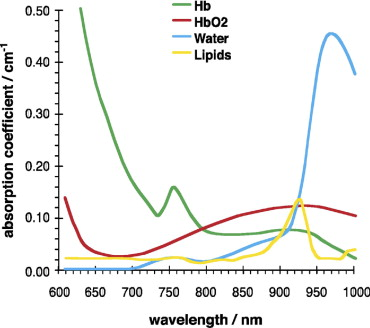
\includegraphics[scale = 1.20]{graphic/window.jpg}}
	\caption{Widma absorpcyjne podstawowych chromoforów tkanek żywych. Charakterystyczne okno optyczne w~zakresie długości fali 650~-~1050~nm}
	\label{rys:window}
	~\\
	(źródło: Na podstawie \cite{Haggblad:2008})
\end{figure}

\subsection{Transluminacja a~metoda refleksyjna}
\label{subsec:TransReflex}

Podczas przeprowadzania procesu prześwietlania lub podświetlania tkanek, szczególnie wówczas, gdy badanie jest długotrwałe, konieczne jest właściwe pozycjonowanie obiektu badanego 
względem układu pomiarowego. Unieruchomienie nie może wpłynąć na stan funkcjonalny badanego ośrodka przy jednoczesnym zachowaniu komfortu. Typowe sposoby pozycjonowania układu 
pomiarowego w~postaci źródeł promieniowania i~detektorów przedstawia rysunek~\ref{rys:position}. 

Przeprowadzanie badań diagnostycznych metodą transluminacji oparte jest o~akwizycję sygnału świetlnego po przejściu przez badany ośrodek, przy ustawieniu detektora 
po przeciwnej stronie obiektu~(rys.~\ref{rys:position}~a). Odebrane promieniowanie optyczne staje się nośnikiem informacji o~charakterystycznych parametrach dotyczących 
właściwości tego obiektu. Diagnostyka spektrofotometryczna przy pomocy metody refleksyjnej możliwa jest dzięki występowaniu rozpraszania wstecznego promieniowania 
świetlnego w~badanym obiekcie biologicznym~\ref{rys:redlight}~b. Promieniowanie w~ośrodku ulega załamaniu, absorpcji oraz wielokrotnemu rozproszeniu, następnie zostaje 
pochłonięte w~detektorze poza ośrodkiem~(rys.~\ref{rys:position}~b,~c). 
\begin{figure}[!ht]
\centerline{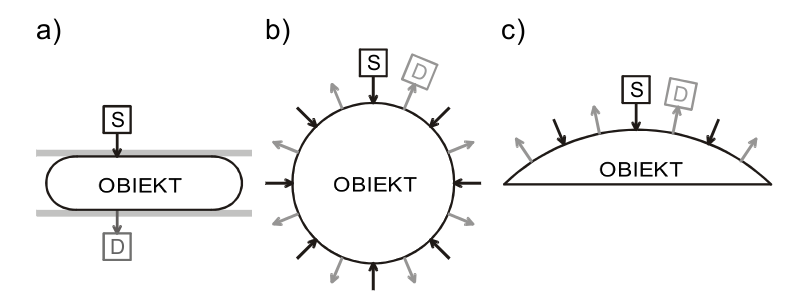
\includegraphics[scale = 0.50]{graphic/position.png}}
	\caption{Metody pozycjonowania badanego obiektu względem układu pomiarowego, S - źródło promieniowania, D - detektor promieniowania}
	\label{rys:position}
	~\\
	(źródło: Na podstawie \cite{Cys:2007})
\end{figure}
\begin{figure}[!ht]
\centerline{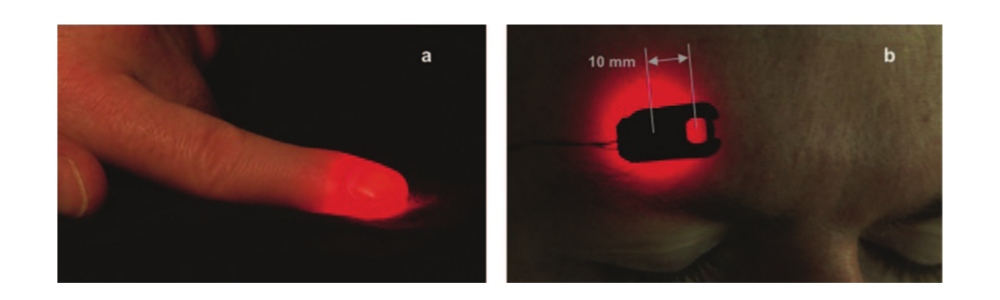
\includegraphics[scale = 0.52]{graphic/redlight.png}}
	\caption{Badanie diagnostyczne przy użyciu światła czerwonego o~długości fali 660 nm metodą transluminacji oraz metodą refleksyjną}
	~\\
	(źródło: Na podstawie \cite{Mann:2007})
	\label{rys:redlight}
\end{figure}

\noindent Natężenie promieniowania wychodzącego z~badanego medium jest wielokrotnie niższe przy zastosowaniu 
metody odbiciowej, gdyż promieniowanie odebrane pochodzi tylko od części promieniowania rozproszonego wstecz. 

\section{Fotopletyzmografia i~pulsoksymetria}
\label{sec:Fotopletyzmografia}

W procesie diagnostyki organizmu żywego ważną rolę odgrywa nieinwazyjne monitorowanie parametrów tętna. Poddając warstwę tkanek promieniowaniu optycznemu, umożliwia się obserwowanie krzywej 
pletyzmograficznej (PPG)~(rys.~\ref{rys:PPG}), której charakterystyczną składową jest fala tętna~\cite{Cys:2007}. Pulsacja krwi tętniczej powoduje niewielkie, cykliczne zmiany objętości 
ośrodka umieszczonego między źródłem a~odbiornikiem. 
\begin{figure}[!ht]
\centerline{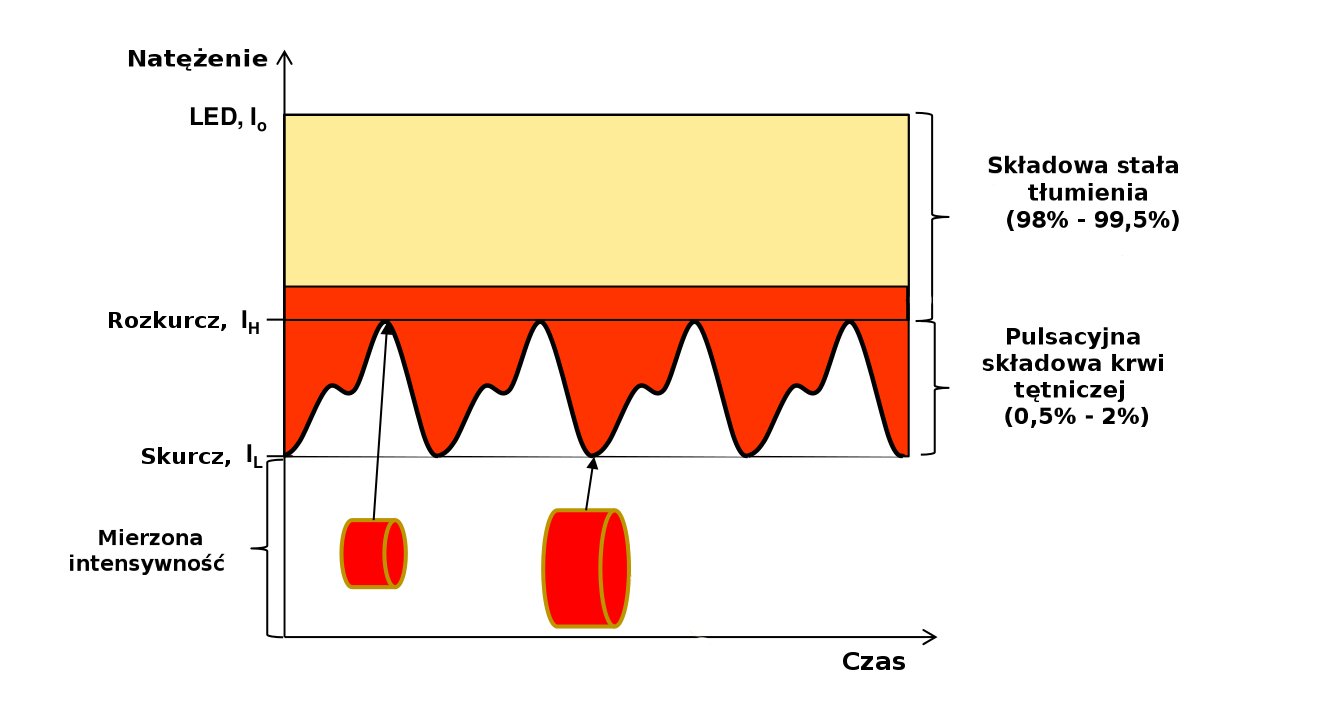
\includegraphics[scale = 0.40]{graphic/PPG.png}}
	\caption{Zmienny przebieg natężenia promieniowania w~następstwie zmian objętości przepływającej krwi w~naczyniach krwionośnych. Wartość natężenia światła osiąga
		 minimum w~chwili przepływu krwi o~najwyższym ciśnieniu}
	~\\
	(źródło: Na podstawie \cite{Dwyer:2008})
	\label{rys:PPG}
\end{figure}
Możliwość detekcji pulsacji tętniczej oraz jej wiarygodne przetworzenie są podstawowym warunkiem realizacji nieinwazyjnego 
optoelektronicznego monitorowania utlenowania krwi tętniczej metodą pulsoksymetrii. W~transmisyjnym wariancie rejestracji sygnałów optycznych występuje, w~porównaniu do wariantu 
odbiciowego, mniejsza wrażliwość na artefakty, niestabilne położenie czujnika oraz inne czynniki zakłócające.

Zgodnie z~zasadami spektrofotometrii, do wykrycia koncentracji $n$ różnych absorberów zawartych w~badanym ośrodku, należy przeprowadzić proces transluminacji dla $n$ różnych długości fali,
przy znanej absorbancji molowej $\alpha(\lambda)$ każdego składnika. Do wykrycia zawartości hemoglobiny ($Hb$) oraz oksyhemoglobiny ($HbO_{2}$) konieczne jest zastosowanie co najmniej
dwóch długości fali, dla których badane substancje wykazują odmienne właściwości optyczne~(rys.~\ref{rys:blood}).
\begin{figure}[ht]
\centerline{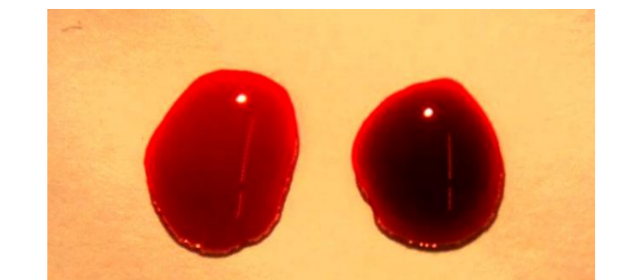
\includegraphics[scale = 0.63]{graphic/blood.png}}
	\caption{Próbki krwi tętniczej oraz krwi żylnej. Różnice w~barwie próbek są skutkiem odmiennych właściwości optycznych hemoglobiny i~oksyhemoglobiny}
	\label{rys:blood}
	~\\
	(źródło: Na podstawie \cite{Dwyer:2008})
\end{figure}

W~celu najgłebszej penetracji promieniowania świetlnego, podczas określania saturacji krwi stosuje się źródła światła o~długościach fali 660~nm oraz 940~nm zawarte w~oknie optycznym tkanek żywych 
(rys.~\ref{rys:RIR}). Fotodetektor stanowi zazwyczaj pojedyncza krzemowa dioda PIN, generująca prąd fotoelektryczny o~wartości proporcjonalnej do natężenia przepuszczonego promieniowania świetlnego. 

Ponieważ częstość zmian objętości naczyń krwionośnych odpowiada częstości skurczów serca, krzywa pletyzmograficzna może być wykorzystana do łatwego wyznaczania tętna. Właściwa częstość 
akcji serca jest równa liczbie globalnych punktów ekstremalnych krzywej PPG w~określonym przedziale czasu.
\begin{figure}[h]
\centerline{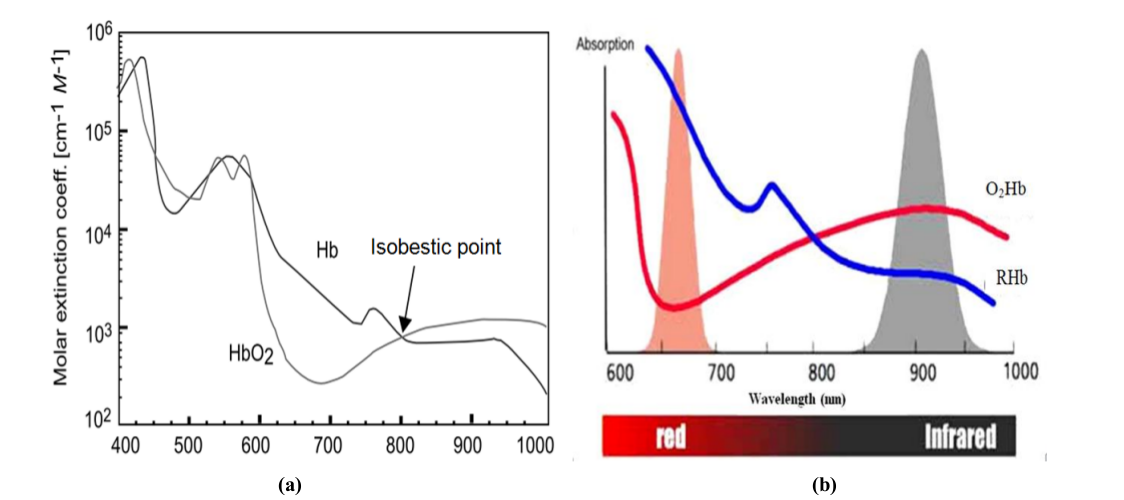
\includegraphics[scale = 0.46]{graphic/RIR.png}}
	\caption{Fragment widma absorpcyjnego hemoglobiny i~oksyhemoglobiny}
	\label{rys:RIR}
	~\\
	(źródło: Na podstawie \cite{Dwyer:2008})
\end{figure}

Pomiar saturacji częściowej $SpO_{2}$ to operacja złożona w~stosunku do pomiaru częstości akcji serca. Natężenie promieniowania odbieranego przy podświetlaniu obiektu złożonego z~tkanek
żywych nie jest wartością stałą w~czasie. Skutkiem istnienia podskórnych naczyń krwionośnych w~postaci tętnic i~żył, krzywa pletyzmograficzna składa się z~dwóch składowych: stałej (DC) oraz zmiennej 
(AC)~(rys.~\ref{rys:maxmin2}). Składowa stała stanowi część promieniowania świetlnego transmitowaną przez warstwę tkanek stałych nie zmieniających znacząco swojej objętości w~przedziale czasu jak: 
kości, skóra, mięśnie, tkanka tłuszczowa~\cite{Fuzzy:2011}.
\begin{figure}[!h]
\centerline{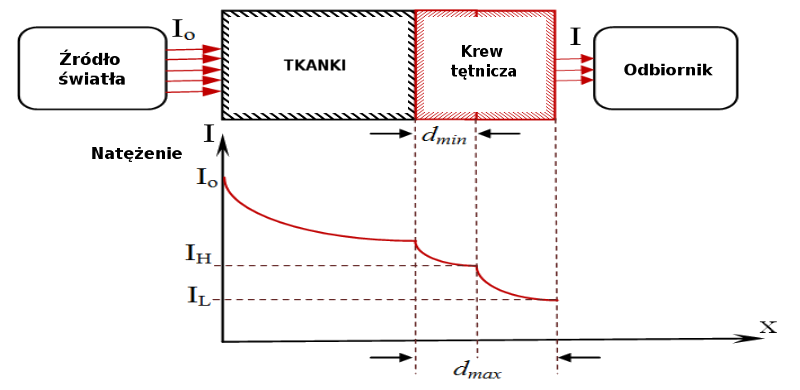
\includegraphics[scale = 0.50]{graphic/maxmin2.png}}
	\caption{Interpretacja wartości minimalnej oraz maksymalnej natężenia promieniowania na podstawie równania Lamberta-Beera}
	\label{rys:maxmin2}
	~\\
	(źródło: Na podstawie \cite{Dwyer:2008})
\end{figure}

W~celu wyznaczenia natężenia promieniowania metodą transluminacji w~tkankach żywych, stosowane jest prawo Lamberta-Beera dla środowiska~niehomogenicznego~(\ref{equ:equ1}).
\begin{equation}
\label{equ:equ1}
	I(t)=I_{0}e^{-(\alpha_{DC}C_{DC}d_{DC}+(\alpha_{Hb}C_{Hb}+\alpha_{HbO_{2}}C_{HbO_{2}})d(t))}
\end{equation}
gdzie:\\
$\alpha_{DC}C_{DC}d_{DC}$ - składowa stała tłumienia tkanek żywych,\\
$\alpha_{Hb}, \alpha_{HbO_{2}}$ - molowy współczynnik absorpcji hemoglobiny i~oksyhemoglobiny,
$C_{Hb}, C_{HbO_{2}}$ - stężenie molowe hemoglobiny i~oksyhemoglobiny.\\

%\noindent Czynnik $(\alpha_{Hb}C_{Hb}+\alpha_{HbO_{2}}C_{HbO_{2}})d(t)$ stanowi składową pulsacyjną  tłumienia. 
\noindent Wartość maksymalna $I_{H}$ oraz minimalna $I_{L}$ natężenia promieniowania odebranego~(rys.~\ref{rys:maxmin1}) wynoszą odpowiednio:
 
\begin{equation}
\label{equ:equ2}
	I_{H}=I_{0}e^{-(\alpha_{DC}C_{DC}d_{DC}+(\alpha_{Hb}C_{Hb}+\alpha_{HbO_{2}}C_{HbO_{2}})d_{H})}
\end{equation}

\begin{equation}
\label{equ:equ3}
	I_{L}=I_{0}e^{-(\alpha_{DC}C_{DC}d_{DC}+(\alpha_{Hb}C_{Hb}+\alpha_{HbO_{2}}C_{HbO_{2}})d_{L})}
\end{equation}
\noindent W~celu uproszczenia i~wyeliminowania funkcji wykładniczej z~równań~(\ref{equ:equ2}) oraz~(\ref{equ:equ3}) obliczamy logarytm naturalny z~ilorazu $I_{H}$ i~$I_{L}$ otrzymując:

\begin{equation}
\label{equ:equ4}
	ln(\frac{I_{H}}{I_{L}})=(\alpha_{Hb}C_{Hb}+\alpha_{HbO_{2}}C_{HbO_{2}})\Delta d
\end{equation}
gdzie:\\
$\Delta d=d_{H}-d_{L}$

\begin{figure}[ht]
\centerline{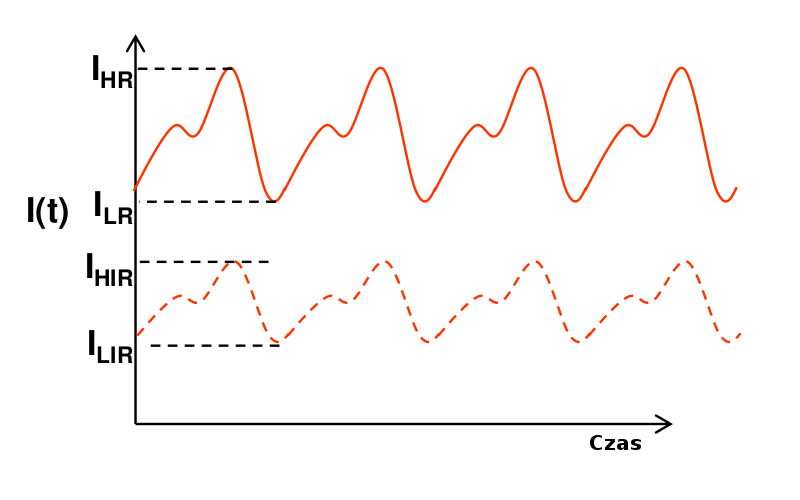
\includegraphics[scale = 0.40]{graphic/maxmin1.png}}
	\caption{Krzywa pletyzmograficzna (PPG) badanego ośrodka dla 660~nm oraz 940~nm}
	\label{rys:maxmin1}
	~\\
	(źródło: Na podstawie \cite{Dwyer:2008})
\end{figure}

\noindent Dla obu długości fali 660~nm oraz 940~nm otrzymano dwa równania z~dwoma niewiadomymi $C_{Hb}$ i~$C_{HbO_{2}}$. Iloraz obu równań oznaczono jako współczynnik~$R$:

\begin{equation}
\label{equ:equ4}
	R=\frac{ln(\frac{I_{HR}}{I_{LR}})}{ln(\frac{I_{HIR}}{I_{LIR}})}=\frac{\alpha_{Hb}(\lambda_{R})C_{Hb}+\alpha_{HbO_{2}}(\lambda_{R})C_{HbO_{2}}}{\alpha_{Hb}C(\lambda_{IR})_{Hb}+\alpha_{HbO_{2}}(\lambda_{IR})C_{HbO_{2}}}
\end{equation}\\
\noindent Przy założeniu, że $\Delta d_{R} = \Delta d_{IR}$.\\ 
\noindent Następnie wyznaczono zawartość procentową hemoglobiny utlenowanej w~całkowitej ilości hemoglobiny~\cite{Fuzzy:2011}.

\begin{equation}
\label{equ:equ4}
	SpO_{2}=\frac{C_{Hb}}{C_{Hb}+C_{HbO_{2}}}~100\%
\end{equation}

\begin{equation}
\label{equ:equ5}
	SpO_{2}=\frac{\alpha_{Hb}(\lambda_{R})-\alpha_{Hb}(\lambda_{IR})R}{\alpha_{Hb}(\lambda_{R})-\alpha_{HbO_{2}}(\lambda_{R})+(\alpha_{Hb}(\lambda_{IR})-\alpha_{HbO_{2}}(\lambda_{IR}))R}~100\%
\end{equation}

\noindent Wyznaczenie teoretycznej wartości wysycenia krwi tętniczej ograniczone zostało do obliczenia parametru $R$~zależnego od wartości maksymalnej i~minimalnej natężenia 
odebranego promieniowania dla obu długości fali~(rys.~\ref{rys:saturation}).

Aproksymacja prawa Lamberta-Beera, eliminująca składową rozpraszania i~odbicia promieniowania na wartość tłumienia ośrodka~(\ref{equ:equ1}), wprowadza błąd pomiarowy w~procesie wyznaczania wysycenia krwi 
tlenem~\cite{Web:1997}. Obliczenia dokonane zostały przy założeniu, że natężenie padającego promieniowania jest sumą natężenia odebranego oraz promieniowania tłumionego w~ośrodku. W~normalnych
warunkach pracy pulsoksymetru, zmierzona wartość nasycenia jest wystarczająca do celów klinicznych, pomimo pominięcia znaczącego tłumienia światła pod wpływem rozpraszania. 

Większość komercyjnych urządzeń do pomiaru wskaźnika $SpO_{2}$ wykorzystuje empiryczną zależność wysycenia krwi od parametru $R$~(rys.\ref{rys:saturation}), wyznaczoną poprzez chemiczną analizę 
składu krwi (in~vitro). Proces kalibracji aparatu pomiarowego eliminuje błędy wprowadzane na skutek uproszczeń dokonanych podczas wyprowadzania teoretycznych zależności.
\begin{figure}[ht]
\centerline{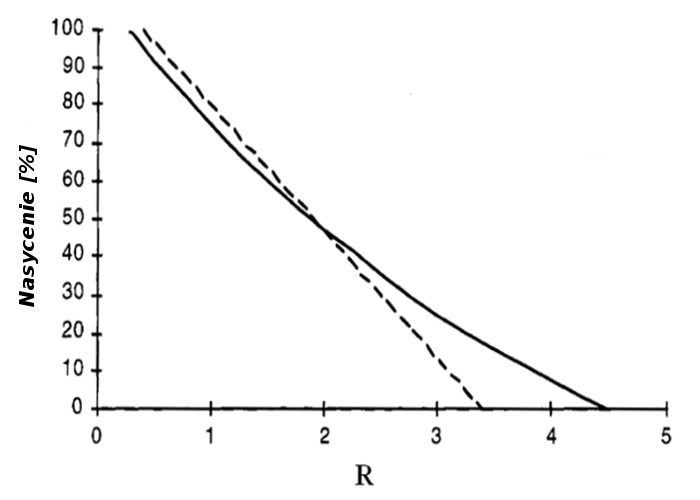
\includegraphics[scale = 0.52]{graphic/saturation.png}}
	\caption{Teoretyczna (linia ciągła) i~empiryczna (linia przerywana) krzywa zależności wskaźnika wysycenia krwi tętniczej tlenem w~funkcji parametru~$R$}
	\label{rys:saturation}
	~\\
	(źródło: Na podstawie \cite{Dwyer:2008})
\end{figure}

\section{Uwarunkowania i~ograniczenia pomiarowe}
\label{sec:Ograniczenia}

Urządzenia monitorujące nasycenie krwi są standardem na oddziałach intensywnej terapii, których niezawodna praca pozwala na właściwą ocenę stanu pacjenta. W~celu uzyskania optymalnej wydajności
i~precyzji, należy wyeliminować czynniki zaburzające warunki przeprowadzanego pomiaru. 

\subsubsection{Ograniczenia fizjologiczne}
\label{subsubsec:fizj}

Wartość wysycenia $SpO2$ jest fizjologicznie związana z~ciśnieniem parcjalnym $PaO2$~\cite{Fuzzy:2011}. Zależność saturacji krwi od wartości $PaO2$ przedstawia rysunek~(rys.\ref{rys:PaO2}).
Wysokim wartościom współczynnika $SpO2$ odpowiadają niewielkie zmiany ciśnienia parcjalnego tlenu. W~zakresie ciśnienia 0-80~mmHg, niewielkie zmiany ciśnienia powodują znaczące wahania
współczynnika saturacji $SpO2$.
\begin{figure}[ht]
\centerline{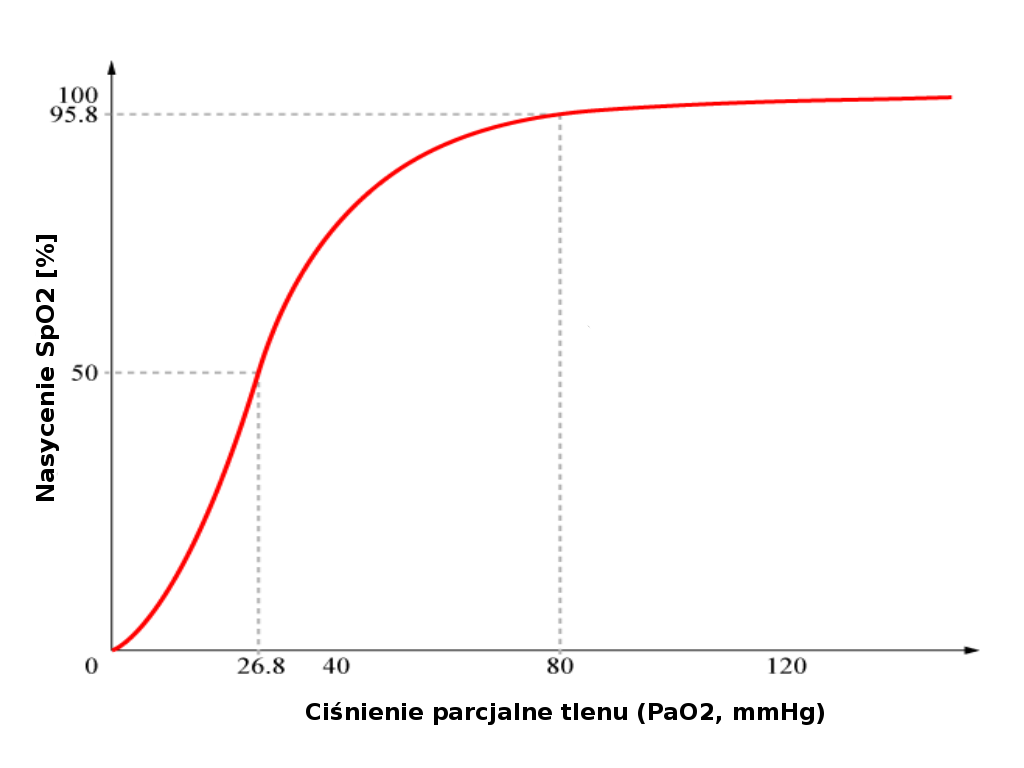
\includegraphics[scale = 0.32]{graphic/PaO2}}
	\caption{Krzywa dysocjacji oksyhemoglobiny. Zależność wysycenia krwi tlenem od ciśnienia parcjalnego $PaO2$}
	\label{rys:PaO2}
	~\\
	(źródło: Na podstawie \cite{Fuzzy:2011})
\end{figure}

Zastosowanie dwóch długości fali w~pomiarach wskaźnika nasycenia krwi, umożliwia określenie stężenia tylko dwóch substancji o~odmiennych właściwościach optycznych. Występowanie związków
hemoglobiny z~tlenkiem węgla, siarką oraz hemoglobiny dysfunkcyjnej powoduje zaburzanie wyniku pomiarów.
Pigmentacja skóry oraz inne absorbery, jak np.~płytka paznokcia, skutecznie tłumią wiązkę promieniowania transmitowanego, co często uniemożliwia uzyskanie odpowiednio silnego sygnału w~odbiorniku.

Płaski kształt czerwonych krwinek powoduje zmianę powierzchni pochłaniania promieniowania podczas skurczu oraz rozkurczu serca~\cite{Fuzzy:2011}. W~chwili skurczu, gdy w~naczyniach 
krwionośnych panuje najwyższe ciśnienie, erytrocyty pod wpływem strumienia przepływającej krwi, ustawiają się prostopadle do kierunku przepływu, zmniejszając aktywną powierzchnię 
absorbującą~(rys.\ref{rys:sysdias}).

\begin{figure}[ht]
\centerline{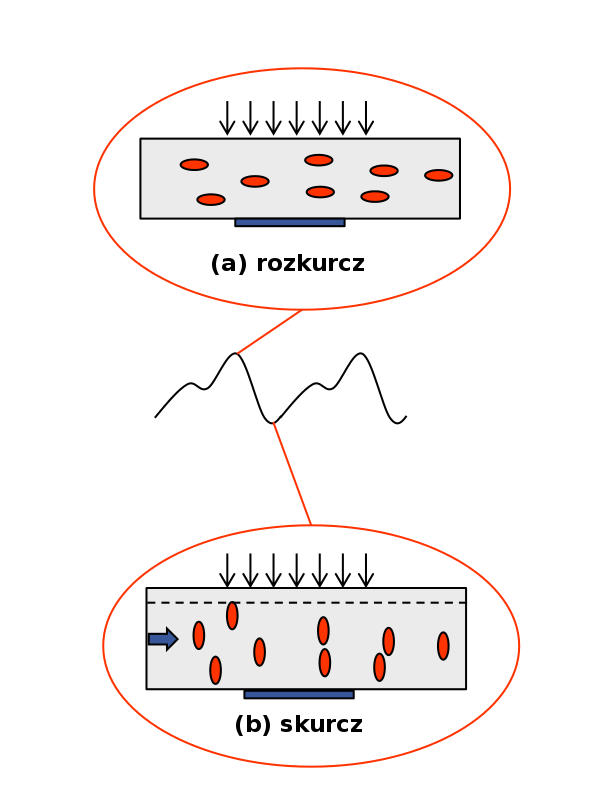
\includegraphics[scale = 0.40]{graphic/sysdias}}
	\caption{Ułożenie krwinek czerwonych podczas skurczu i~rozkurczu serca}
	\label{rys:sysdias}
	~\\
	(źródło: Na podstawie \cite{Fuzzy:2011})
\end{figure}

\subsubsection{Ograniczenia związane z przetwarzaniem sygnałów}
\label{subsubsec:fizj}

Najpoważniejszym zagrożeniem podczas przetwarzania sygnałów dostarczonych z~detektora promieniowania są zakłócenia spowodowane ruchem mierzonego obiektu umieszczonego
w~klipsie pulsoksymetru~(rys.\ref{rys:noise}). Użyteczny sygnał zawierający pulsującą składową tętna jest wielokrotnie słabszy od powstających zakłóceń. W~celu uniknięcia
zniekształceń sygnału użytecznego, pomiar saturacji krwi powinien przebiegać przy całkowitym unieruchomieniu kończyny, na której znajduje się klips pomiarowy.

\begin{figure}[ht]
\centerline{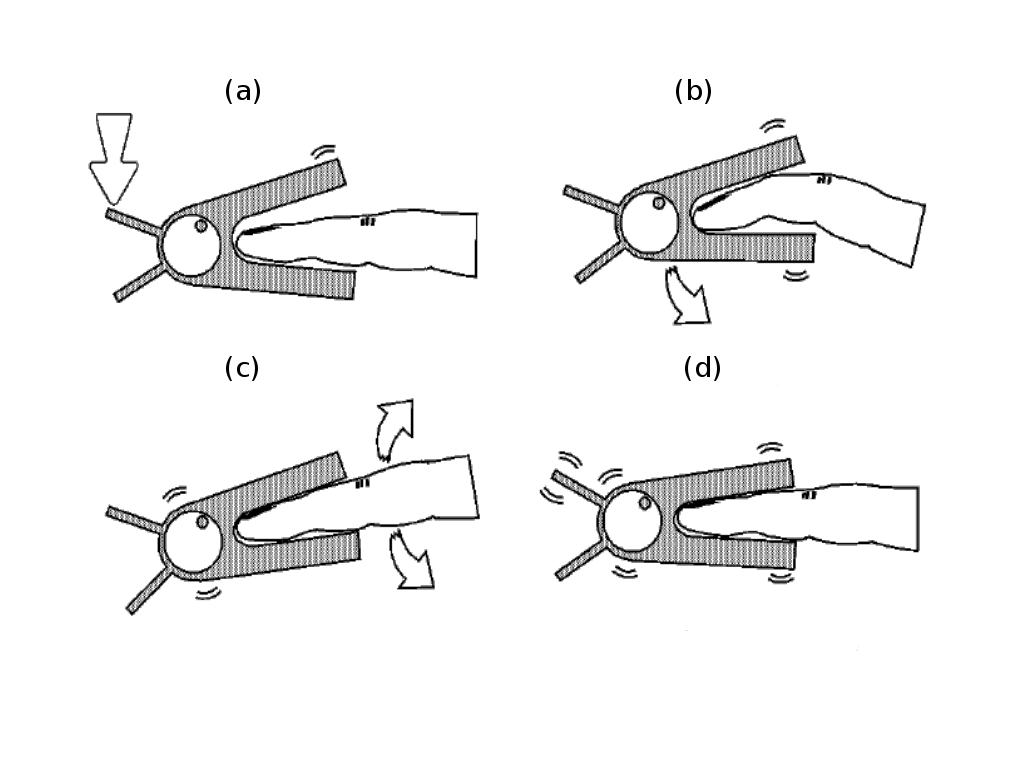
\includegraphics[scale = 0.38]{graphic/noise}}
	\caption{Przykłady nieprawidłowego umieszczenia palca w~klipsie pomiarowym: nieprawidłowe dociśnięcie klipsa~(a), zginanie obiektu~(b), poruszanie obiektu wraz z~klipsem~(c)
		oraz drgania obiektu wraz z~klipsem~(d)}
	\label{rys:noise}
	~\\
	(źródło: Na podstawie \cite{Dwyer:2008})
\end{figure}

Przedstawiona metodyka pomiaru wysycenia krwi została opracowana przy założeniu, że składowa pulsacyjna krzywej pletyzmograficznej jest związana tylko i~wyłącznie z~przepływem krwi tętniczej.
W~rzeczywistości, powracająca krew żylna wprowadza dodatkową składową zmienną o~niewielkiej amplitudzie~(rys.\ref{rys:vein}). Sposób wyznaczania saturacji $SpO2$ opiera się na analizie amplitudowej 
sygnału zmiennego, otrzymanego w~procesie transluminacji. Skutkiem występowania składowej zmiennej odtlenowanej krwi żylnej (saturacja 65\%~-~75\%) jest wprowadzenie błędu pomiarowego w~procesie 
wyznaczania prawidłowego współczynnika wysycenia krwi tętniczej~\cite{Fuzzy:2011}. 

\begin{figure}[h]
\centerline{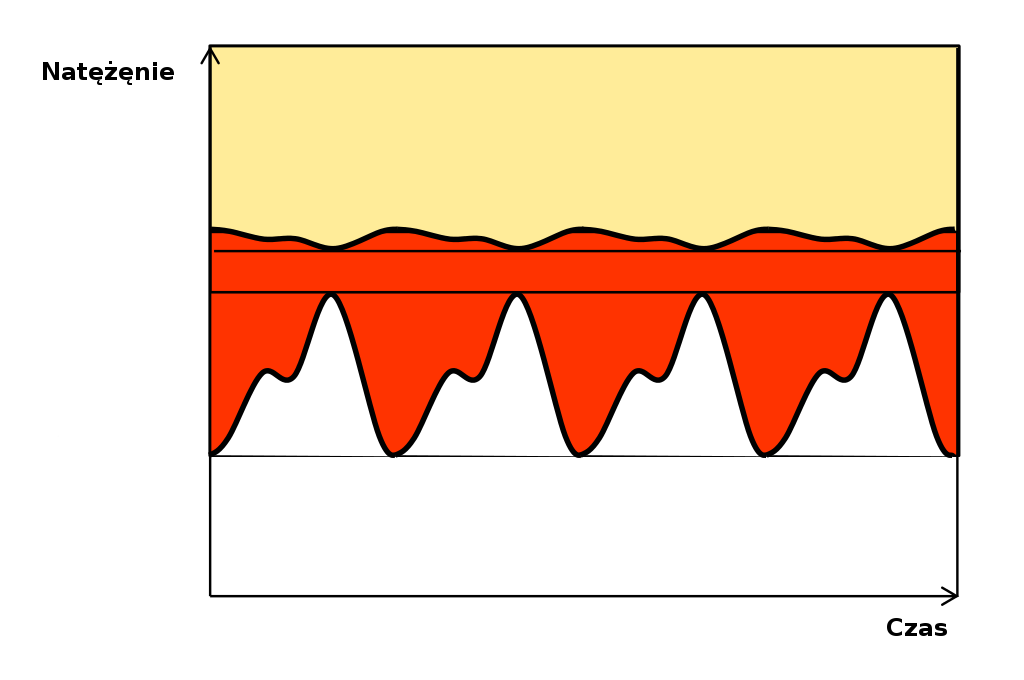
\includegraphics[scale = 0.36]{graphic/vein}}
	\caption{Krzywa pletyzmograficzna (PPG) krwi tętniczej wraz ze składową zmienną krwi żylnej}
		
	\label{rys:vein}
	~\\
	(źródło: Na podstawie \cite{Dwyer:2008})
\end{figure}

Poważnym problemem pomiarowym jest wpływ obcego promieniowania występującego w~sąsiedztwie stanowiska pomiarowego. W~przeciwieństwie do natężenia promieniowania stałego w~czasie, najpoważniejszym 
problemem jest promieniowanie pochodzące od źródeł światła zasilanych bezpośrednio z~sieci~energetycznej. 
Pojawienie się składowej zmiennej o~częstotliwości 50~-~60~Hz w~sąsiedztwie widma częstotliwościowego sygnału użytecznego, narzuca konieczność stosowania filtrów dolnoprzepustowych o~stromych zboczach 
w~celu uniknięcia degradacji~sygnału użytecznego.


\renewcommand{\figurename}{Rys.}

\chapter{Sprzętowa realizacja układu pomiarowego}
\label{cha:Sprzęt}

\fontsize{14}{15}\selectfont

%---------------------------------------------------------------------------
Optyczna metoda wyznaczania nasycenia krwi tętniczej tlenem oraz tętna bazuje na analizie krzywej pletyzmograficznej, uzyskanej w~procesie transluminacji tkanek przy zastosowaniu dwóch długości fali.
Odpowiednimi źródłami fal elektromagnetycznych w~zakresie promieniowania widzialnego i~bliskiej podczerwieni są ogólnodostępne diody elektroluminescencyjne, emitujące promieniowanie w~wąskim 
zakresie częstotliwości. Detekcja sygnału użytecznego w~procesie prześwietlania odbywa się przy pomocy fotodiody, która pracując jako źródło prądowe, generuje prąd wprost proporcjonalny do 
padającego promieniowania. Fotoprąd niosący użyteczną informację dla procesu pulsoksymetrii, trafia do układów konwersji, gdzie zostaje zamieniony na łatwiejszy w~użyciu sygnał napięciowy. Dalej 
przeprowadzany jest proces filtracji oraz kondycjonowania, aby ostatecznie poprzez przetwornik analogowo~-~cyfrowy sygnał napięciowy mógł być wykorzystany przez system mikroprocesorowy 
w~celu wyznaczenia poszukiwanych parametrów i~wskaźników.

Schemat komercyjnego aparatu pomiarowego przedstawia rysunek~\ref{rys:Schematic}. Nowoczesne rozwiązania w~postaci rozbudowanych układów wbudowanych dostarczają szerokiej funkcjonalności 
zapewniając wygodę użytkowania. Zasilanie bateryjne, wyświetlacze LCD, panele dotykowe oraz łatwy w~użyciu interfejs~użytkownika umożliwiają przeprowadzanie pomiarów przez pacjenta w~dowolnym 
miejscu bez pomocy operatora.
\begin{figure}[!h]
	\centerline{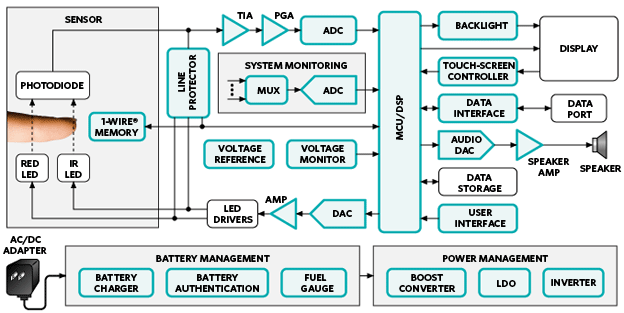
\includegraphics[scale = 0.76]{graphic/Schematic}}
	\caption{Schemat blokowy komercyjnego aparatu pomiarowego}
	~\\
	(źródło: http://www.maximintegrated.com)
	\label{rys:Schematic}
\end{figure}

W~niniejszej pracy zrealizowane zostaną elementy układu, niezbędne do wykonania pomiarów szukanych parametrów częstości akcji serca i~saturacji. Zakres prac wykonywanych przez autora projektu
zawiera schemat na rysunku~\ref{rys:MySchematic}.
\begin{figure}[!h]
	\centerline{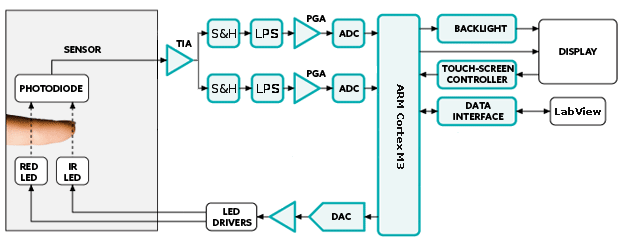
\includegraphics[scale = 0.76]{graphic/MySchematic}}
	\caption{Schemat blokowy pulsoksymetru wykonywanego w~ramach pracy}
	~\\
	(źródło: http://www.maximintegrated.com)
	\label{rys:MySchematic}
\end{figure}


\section{Układ sterowania natężeniem promieniowania LED}
\label{sec:LedSterownik}

Źródła światła w~postaci diod elektroluminescencyjnych generują promieniowanie, którego natężenie jest wprost proporcjonalne do prądu przepływającego przez obszar aktywny złącza P-N~(rys.~\ref{rys:LED}).
Najprostszym sposobem regulacji natężenia promieniowania jest szeregowe połączenie diody z~układem źródła prądowego sterowanego napięciowo, umożliwiającego liniową regulację przepływającego prądu. Możliwość 
płynnej regulacji intensywności światła umożliwia dostosowanie punktu pracy diody do grubości i~struktury badanego obiektu oraz umożliwia kompensowanie nierównomiernej charakterystyki czułości fotodiody~(rys.~\ref{rys:BPW34}).
\begin{figure}[!ht]
	\centerline{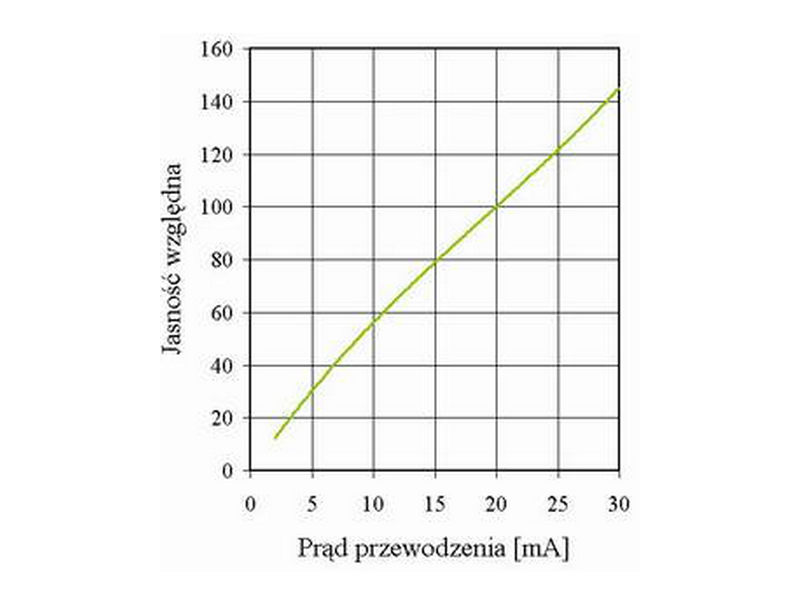
\includegraphics[scale = 0.46]{graphic/LED}}
	\caption{Zależność względnego natężenia promieniowania diody od przepływającego prądu przewodzenia}
	~\\
	(źródło: http://www.lediko.com)
	\label{rys:LED}
\end{figure}

\begin{figure}[!ht]
	\centerline{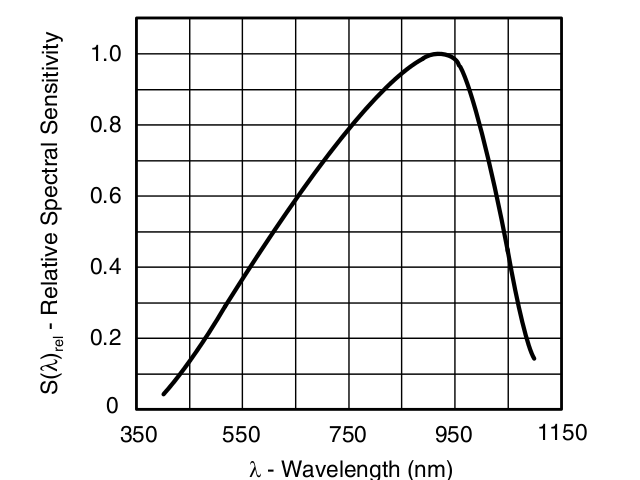
\includegraphics[scale = 0.46]{graphic/BPW34}}
	\caption{Względna charakterystyka czułości fotodiody PIN typu BPW34}
	~\\
	(źródło: na podstawie \cite{BPW34})
	\label{rys:BPW34}
\end{figure}

Przykład sterowanego źródła prądowego wykorzystanego w~projekcie pulsoksymetru przedstawiono na rysunku~\ref{rys:Led_Control}a. Zastosowanie wzmacniacza operacyjnego powoduje zwiększenie impedancji
wejściowej, co skutecznie zmniejsza obciążenie źródła sygnału sterującego. Pętla ujemnego sprzężenia zwrotnego obejmująca złącze emiter-baza tranzystora bipolarnego umożliwia liniową regulację
prądu wyjściowego przy pomocy napięcia sterującego. Duże wzmocnienie wzmacniacza operacyjnego oraz istnienie pętli ujemnego sprzężenia zwrotnego powodują powstanie masy pozornej pomiędzy wejściami wzmacniacza. 
Przy założeniu równych potencjałów na obu wejściach wzmacniacza uzyskujemy następujące równanie napięciowego prawa Kirchoffa: 
\begin{equation}
\label{equ:Kirchoff1}
	V_{IN} - V_{R_{1}} = 0,	
\end{equation}
gdzie:\\
$V_{R_{1}} = IR_{1}$

\begin{equation}
\label{equ:Kirchoff2}
	I = \frac{V_{IN}}{R_{1}}
\end{equation}

Metoda pomiarowa zakłada detekcję natężenia promieniowania pochodzącego od dwóch źródeł promieniowania, przy czym niedozwolona jest sytuacja równoczesnego zasilania źródeł światła w~określonej chwili czasowej.
W~tym celu równolegle do diody elektroluminescencyjnej dodano tranzystor polowy MOSFET z~kanałem typu~P stanowiący prosty układ kluczujący~(rys:~\ref{rys:Led_Control}b).
\begin{figure}[ht]
	\centerline{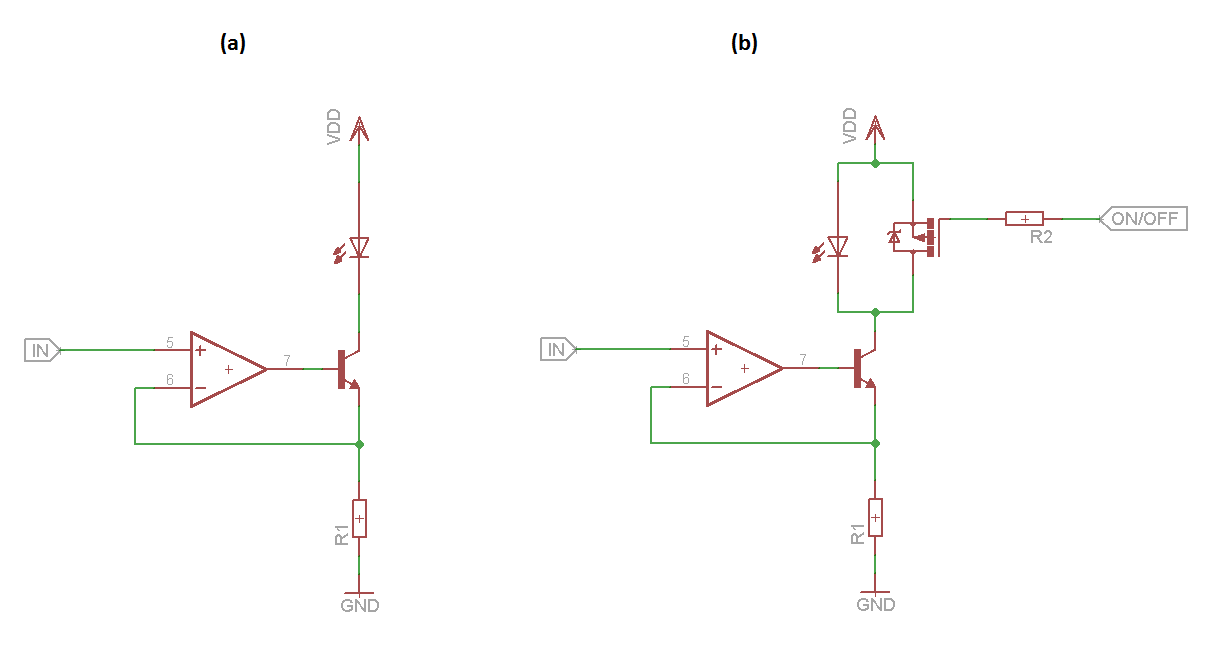
\includegraphics[scale = 0.58]{graphic/Led_Control}}
	\caption{Dioda LED zasilana źródłem prądowym sterowanym napięciowo}
	~\\
	(źródło: Schemat PCB)
	\label{rys:Led_Control}
\end{figure}

Sterując odpowiednio napięciem bramki, tranzystor polowy wprowadzany jest w~stan całkowitego otwarcia lub w~stan zatkania. W~stanie otwarcia cały prąd źródła płynie przez otwarty kanał tranzystora 
uniemożliwiając zasilenie diody. Tranzystory stanowiące przełączane klucze uruchamiane są naprzemiennie z~częstotliwością 1~kHz. 

Zakres liniowej regulacji prądu napięciem sterującym $V_{IN}$ ograniczony jest stanem nasycenia tranzystora bipolarnego. Wartość maksymalnego napięcia sterującego, dla którego tranzystor 
znajduje się w~stanie nasycenia wynosi:
\begin{equation}
\label{equ:Saturation1}
	V_{IN_{max}} = V_{DD} - V_{D} - V_{CES}
\end{equation}
gdzie:\\
$V_{CES}$ - napięcie nasycenia złącza emiter-kolektor,\\
$V_{D}$ - napięcie na diodzie elektroluminescencyjnej. 

\subsubsection{Sonda pomiarowa pulsoksymetru}
\label{subsubsec:Sonda}

Proces prześwietlania tkanek żywych metodą transluminacji, dokonywany jest poprzez poddanie promieniowaniu silnie ukrwionych i~stosunkowo cienkich fragmentów ciała, takich jak końcówki palców oraz 
płatki uszu. W~niniejszej pracy skupiono się na wariancie prześwietlania palców w~miejscach występowania płytek paznokci. W~celu zapewnienia odpowiednich warunków pomiaru oraz komfortu badanej osoby 
zastosowano dedykowaną sondę pomiarową w~formie zaciskanego klipsa umieszczanego na palcach~(rys:~\ref{rys:Sonda}).
Sonda wyposażona jest w~diody LED emitujące promieniowanie w~zakresie 660~nm i~940~nm oraz fotodiodę PIN, której charakterystyka czułości obejmuje obie długości fali. Przewód łączący sondę z~urządzeniem
pomiarowym zawiera ekran minimalizujący wpływ zakłóceń zewnętrznych na użyteczny sygnał prądowy fotodiody.
\begin{figure}[ht]
	\centerline{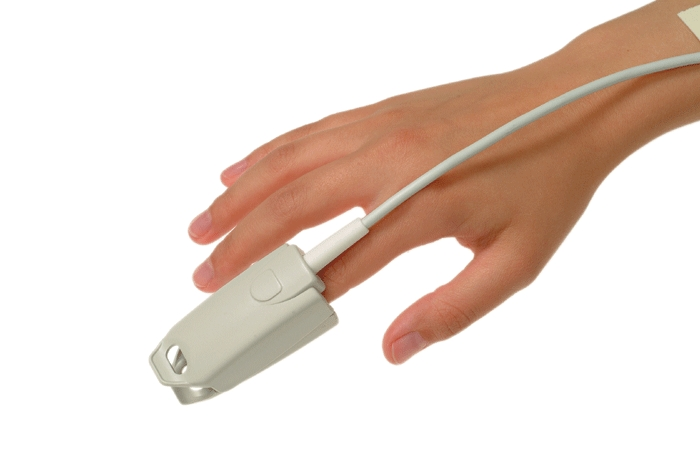
\includegraphics[scale = 0.45]{graphic/sensor}}
	\caption{Sonda pomiarowa pulsoksymetru do badania metodą transluminacji}
	~\\
	(źródło: http://www.covidien.com)
	\label{rys:Sonda}
\end{figure}

\section{Konwerter prąd - napięcie}
\label{sec:LedSterownik}

Celem konwertera jest zamiana sygnału prądowego płynącego ze źródła w~postaci fotodiody na znacznie wygodniejszy z~punktu widzenia dalszej analizy sygnał napięciowy. Uzyskany sygnał w~postaci napięcia 
zmiennego jest poddawany dalszej filtracji i~wzmocnieniu. 
Układ wzmacniacza transimpedancyjnego TIA (ang.~Transimpedance Amplifier) charakteryzuje się bardzo małą rezystancją wejściową. Może on współpracować tylko ze źródłami prądowymi (o dużej rezystancji wewnętrznej), 
ponieważ jego wejście stanowi masę pozorną. 
Wartość prądu wejściowego $I$ nie zależy wówczas od parametrów układu konwertera, ale od źródła sygnału wejściowego~\cite{Rako}. Rysunek~(\ref{rys:IU}) przedstawia schemat konwertera $I/V$.
\begin{figure}[ht]
	\centerline{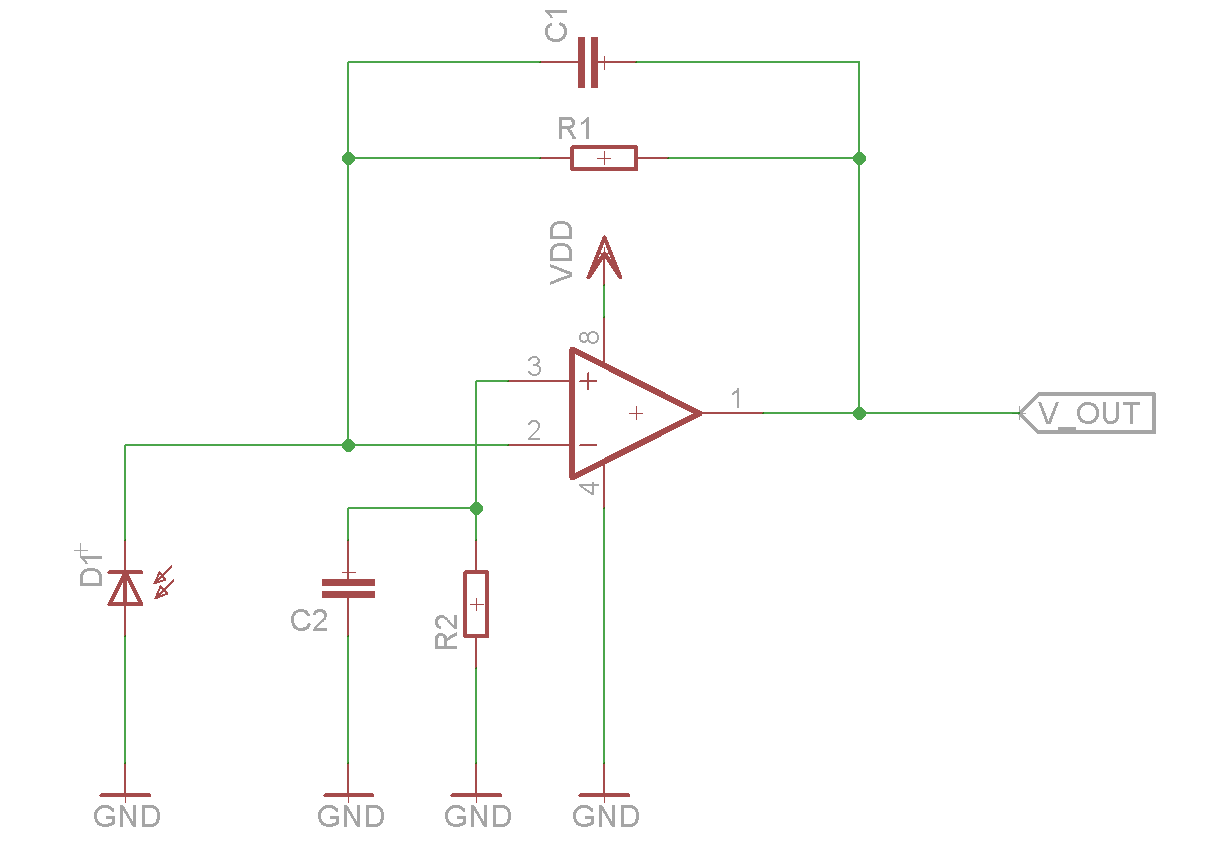
\includegraphics[scale = 0.42]{graphic/IU}}
	\caption{Schemat ideowy konwertera prąd - napięcie na bazie wzmacniacza operacyjnego}
	~\\
	(źródło: Schemat PCB)
	\label{rys:IU}
\end{figure}

Wzmacniacz operacyjny objęty jest pętlą ujemnego sprzężenia zwrotnego, której skutkiem jest istnienie masy pozornej pomiędzy wejściem odwracającym a~wejściem nieodwracającym wzmacniacza. 
Sprzężenie zwrotne realizowane jest za pośrednictwem rezystancji $R_{1}$. Wartość napięcia wyjściowego jest wprost proporcjonalna do prądu wejściowego, a~współczynnik proporcjonalności stanowi rezystancja $R_{1}$.
\begin{equation}
\label{equ:IU}
	V_{OUT} = I_{IN}R_{1}	
\end{equation}

Projektując konwerter prąd - napięcie, autor pracy dużą uwagę skupił na doborze odpowiedniego wzmacniacza operacyjnego o~niskich wejściowych prądach polaryzujących, które sumują się z~sygnałem użytecznym. 
Im mniejsze wartości prądów polaryzujących, tym mniejszy jest błąd przesunięcia napięcia wyjściowego. W~projekcie zastosowano wzmacniacze operacyjne MAXIM MAX4489 o~wejściowych prądach polaryzujących z~przedziału 
1~-~150~pA.

Rozróżnia się dwie metody łączenia źródła fotoprądu w~postaci fotodiody z~układem wzmacniacza transimpedancyjnego. Ze względu na rodzaj odbieranego sygnału należy dokonać wyboru pomiędzy szybkością 
odpowiedzi układu a~precyzją sygnału wyjściowego. Dobór odpowiedniej konfiguracji pracy fotodiody uwarunkowany jest istnieniem pojemności złączowej diody pracującej w~trybie polaryzacji wstecznej~\cite{Rako}. 
Model zastępczy fotodiody półprzewodnikowej przedstawiono na rysunku~\ref{rys:modelPIN}. 

\begin{figure}[ht]
	\centerline{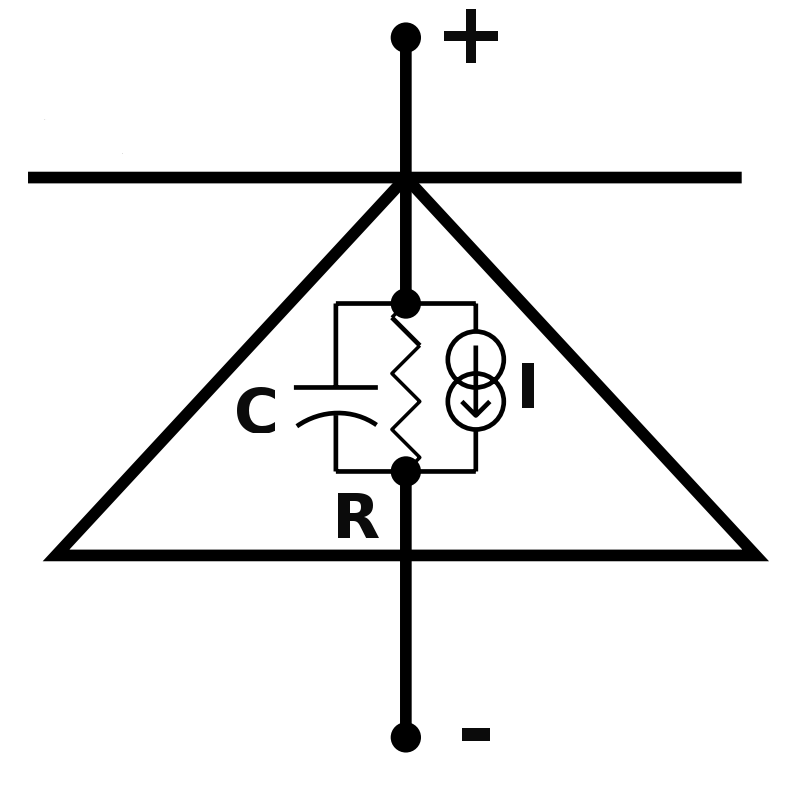
\includegraphics[scale = 0.22]{graphic/modelPIN}}
	\caption{Model fotodiody pracującej w~trybie rewersyjnym}
	~\\
	(źródło: na podstawie \cite{Rako})
	\label{rys:modelPIN}
\end{figure}

Cechą pojemności $C$ złącza P-N jest zmiana jej wartości pod wpływem przyłożonego napięcia rewersyjnego. Wraz ze wzrostem napięcia w~kierunku zaporowym rozszerza się warstwa zubożona stanowiąca dielektryk
kondensatora. Zwiększająca się grubość obszaru zubożonego powoduje zmniejszenie pojemności fotodiody, zmniejszając tym samym czas odpowiedzi fotodiody na impuls promieniowania. Równoległy symbol 
rezystancji $R$ w~modelu symbolizuje prąd ciemny, którego wartość zwiększa się wraz ze wzrostem napięcia na fotodiodzie~\cite{Rako}. 

Ze względu na istnienie powyższych elementów modelu fotodiody rozróżniono fotowoltaiczny i~fotokonduktancyjny tryb pracy~(rys.~\ref{rys:photocond}).
\begin{figure}[ht]
	\centerline{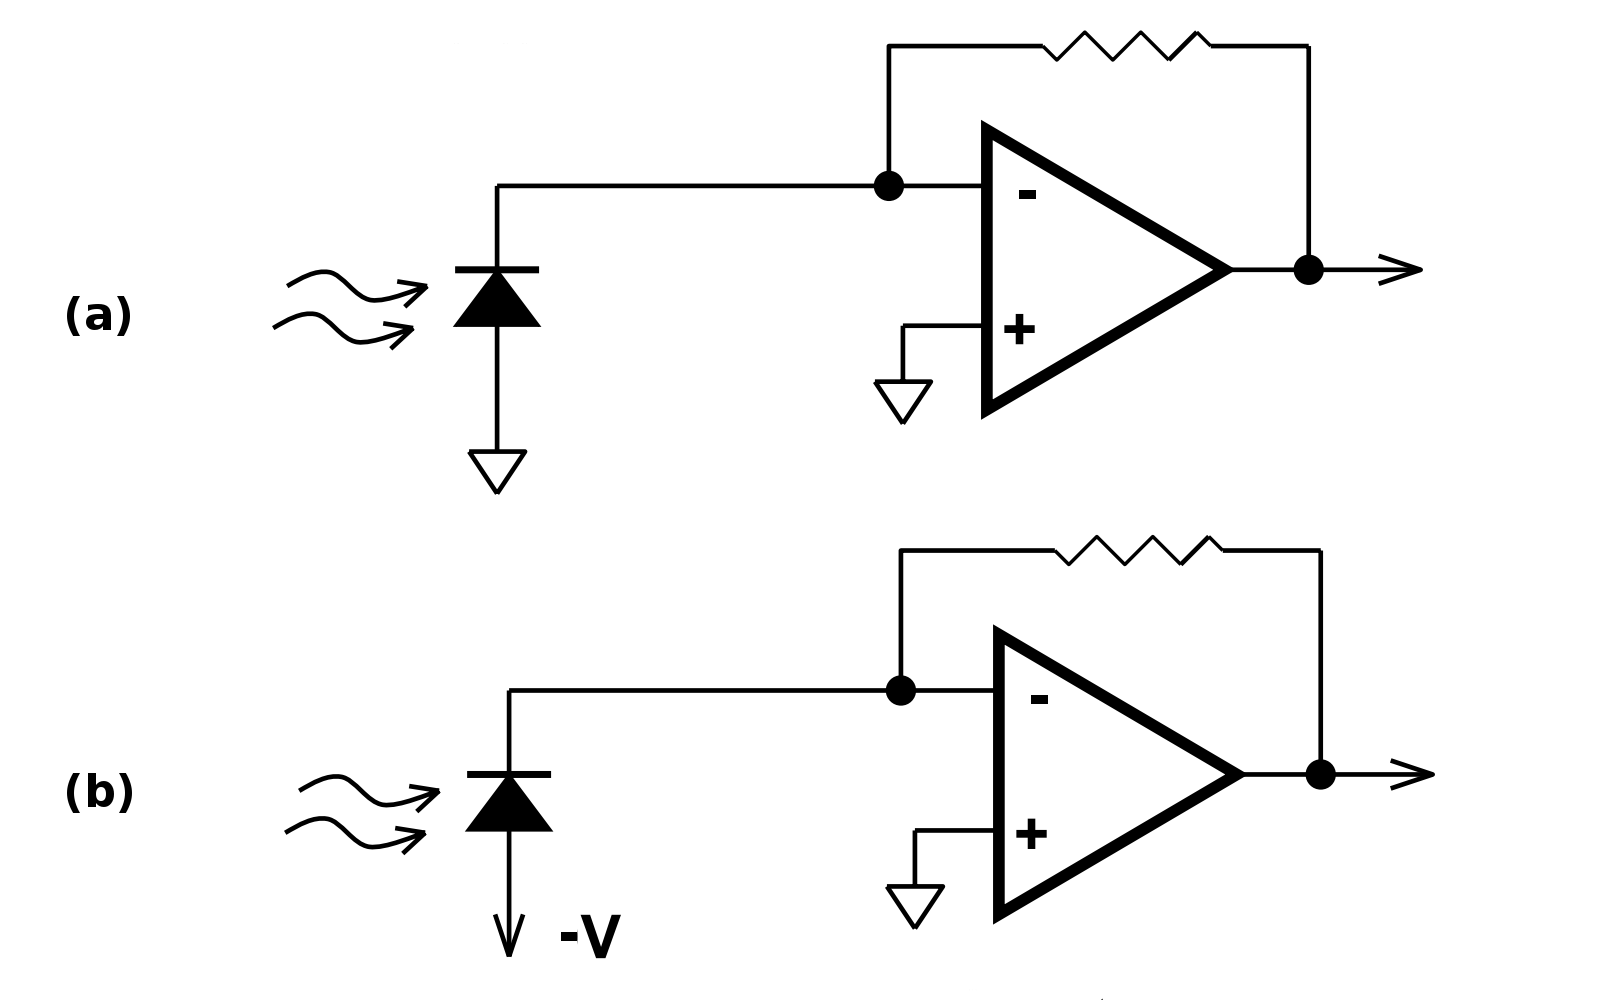
\includegraphics[scale = 0.2]{graphic/photocond}}
	\caption{Tryby pracy fotodiody ze wzmacniaczem transimpedancyjnym: (a) tryb fotowoltaiczny, (b) tryb fotokonduktancyjny}
	~\\
	(źródło: na podstawie \cite{Rako})
	\label{rys:photocond}
\end{figure}

\noindent W~trybie fotowoltaicznym napięcie rewersyjne diody stanowi różnica potencjałów pomiędzy wejściem odwracającym wzmacniacza a~potencjałem masy układu. W~konfiguracji wzmacniacza objętego pętlą ujemnego 
sprzężenia zwrotnego na wejściu odwracającym istnieje masa pozorna. Zatem napięcie rewersyjne diody jest równe wejściowemu napięciu niezrównoważenia. Napięcie to zależy od modelu wzmacniacza operacyjnego 
oraz konkretnego egzemplarza~\cite{Gorecki:2004}.

\noindent Tryb pracy fotowoltaicznej cechuje pomijalnie mała wartość prądu ciemnego rzędu $\mu$A oraz niski poziom szumów, co jest decydujące podczas precyzyjnej detekcji małych sygnałów. W~przypadku trybu fotokonduktancyjnego 
mała pojemność złączowa diody umożliwia pracę z~szybkimi sygnałami o~stromych zboczach~\cite{Rako}. 
W~niniejszym projekcie zastosowano wariant pracy fotowoltaicznej ze względu na detekcję wolnozmiennego sygnału tętna o~niewielkiej amplitudzie.


\subsubsection{Kompensacja częstotliwościowa konwertera $I/V$ }
\label{subsubsec:kompensacja}

Konwerter prąd - napięcie z~rezystorem w~pętli ujemnego sprzężenia zwrotnego jest najprostszą realizacją wzmacniacza transimpedancyjnego (TIA). Pomimo prostoty układu, w~celu zapewnienia poprawnej
pracy wzmacniacza należy dokonać wyboru pomiędzy parametrami, takimi jak poziom szumów, napięcie offsetu, pasmo przenoszenia oraz stabilność. Stabilność głównie jest parametrem kluczowym podczas 
konwersji~\cite{Bhat:2012}.
Układ wzmacniacza transimpedancyjnego, z~pętlą ujemnego sprzężenia zwrotnego podatny jest na oscylacje napięcia wyjściowego. Podatność układu konwertera $I/V$ wynika z~istnienia pojemności
złączowej fotodiody pracującej w~stanie rewersyjnym. W~celu uniknięcia niepożądanych zakłóceń sygnału wyjściowego, układ wzmacniacza kompensowany jest poprzez zastosowanie dodatkowej pojemności $C_{1}$
bocznikującej rezystancję pętli sprzężenia~\cite{Rako}.


\section{Układ próbkująco - pamiętający (Sample and Hold)}
\label{sec:SampleHold}

Multipleksowane sygnały pochodzące od dwóch niezależnych źródeł promieniowania poddawane są detekcji na wspólnym elemencie detekcyjnym oraz wspólnym konwerterze prąd - napięcie. Każdy z~sygnałów jest następnie osobno filtrowany, 
wzmacniany oraz ostatecznie próbkowany w~przetworniku analogowo - cyfrowym. W~związku z~zastosowaniem pojedynczego układu wzmacniacza transimpedancyjnego, niezbędną czynnością okazuje się ponowne
rozdzielenie obu multipleksowanych sygnałów. 
Powyższe wymagania spełnia układ próbkująco - pamiętający, podtrzymujący spróbkowany poziom napięcia na wyjściu konwertera $I/V$~(rys.~\ref{rys:SampleHold}). 

\begin{figure}[ht]
	\centerline{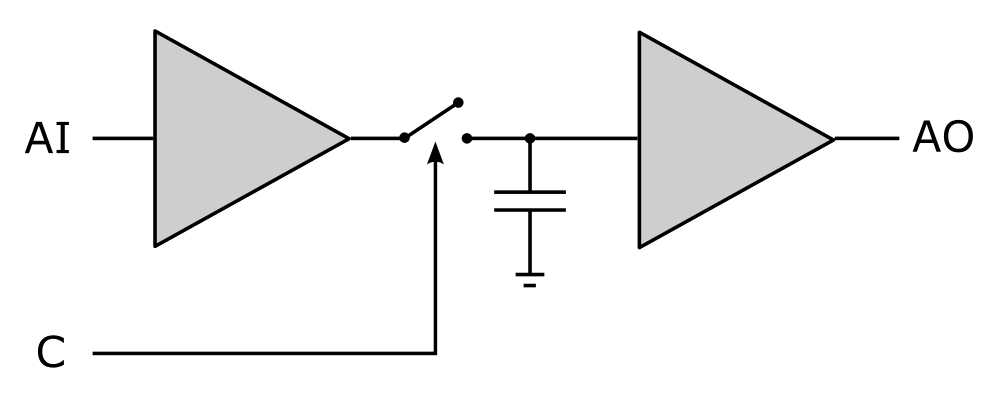
\includegraphics[scale = 0.3]{graphic/SampleHold}}
	\caption{Układ próbkująco~-~pamiętający podtrzymujący napięcie zatrzaśnięte w~chwili próbkowania}
	~\\
	(źródło: http://www.interfacebus.com)
	\label{rys:SampleHold}
\end{figure}

Bufory układu zrealizowano przy pomocy wzmacniacza operacyjnego z~pętlą sprzężenia zwrotnego w~konfiguracji wtórnika napięcia. W~roli elementu kluczującego zastosowano klucz analogowy w~postaci układu scalonego
CMOS 4066. Układ kluczujący zbudowany w~technice CMOS umożliwia przełączanie sygnałów analogowych zbliżonych poziomem zarówno do dodatniej, jak i~ujemnej szyny zasilania~(rys.~\ref{rys:4066}).
\begin{figure}[ht]
	\centerline{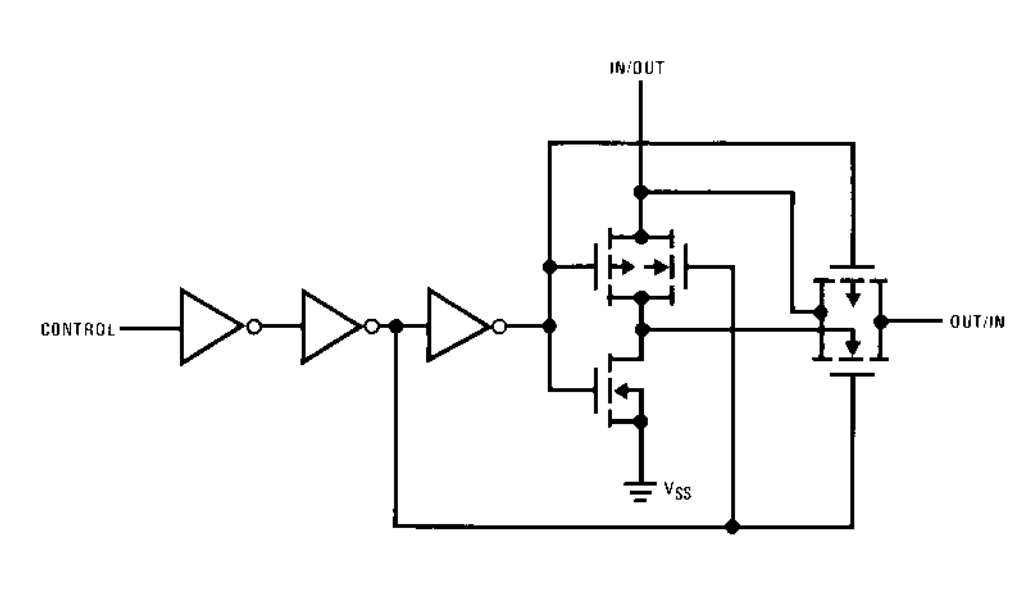
\includegraphics[scale = 0.4]{graphic/4066}}
	\caption{Schemat klucza analogowego układu scalonego CMOS 4066}
	~\\
	(źródło: na podstawie\cite{4066})
	\label{rys:4066}
\end{figure}

Podanie wysokiego stanu logicznego na wejście sterujące klucza analogowego powoduje ładowanie pojemności podtrzymującej do napięcia wejściowego. Zadaniem kondensatora jest podtrzymanie poziomu napięcia
w czasie, gdy klucz jest wyłączony. W~roli bufora napięcia na kondensatorze zastosowano układ wtórnika napięcia o~wysokoimpedancyjnych wejściach nie stanowiących znaczącego obciążenia dla pojemności. 
Nieodłącznym efektem próbkowania sygnałów analogowych jest powstawanie charakterystycznego szumu w~postaci przebiegu schodkowego, związanego ze skończoną wartością częstotliwości sygnału 
kluczującego~(rys.~\ref{rys:samples}).  

\begin{figure}[ht]
	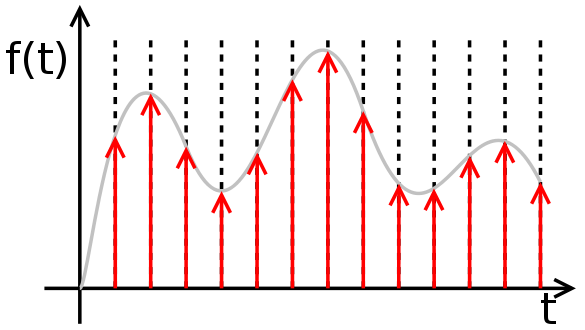
\includegraphics[scale = 0.35]{graphic/sample}
	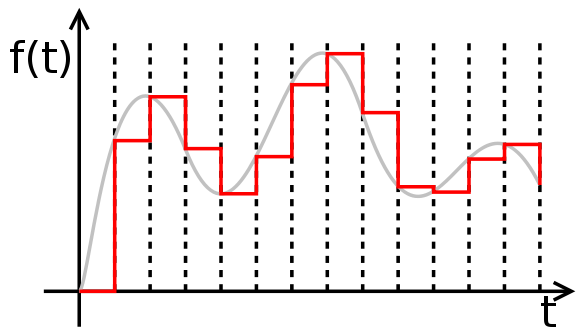
\includegraphics[scale = 0.35]{graphic/sample_hold}
	\caption{Zasada działania układu próbkująco~-~pamiętającego. Charakterystyczny przebieg schodkowy będący efektem próbkowania sygnału analogowego}
	~\\
	(źródło: na podstawie\cite{4066})
	\label{rys:samples}
\end{figure}

W~celu zminimalizowania wpływu szumu próbkowania na dalszy proces analizy sygnału zastosowano wielokrotne zwiększenie częstotliwości próbkowania w~stosunku do częstotliwości sygnału $PPG$, zwane nadpróbkowaniem. 
W~efekcie uzyskuje się przesunięcie widma szumu próbkowania w~kierunku wyższych częstotliwości, co znacznie ułatwia filtrowanie szumu bez degradacji sygnału użytecznego.

\section{Układ filtrujący w~konfiguracji Sallen-Key}
\label{sec:SallenKey}

Szum będący efektem demultipleksacji sygnału w~układzie próbkująco~-~pamiętającym oraz pozostałe szumy generowane przez otoczenie obiektu badanego, w~tym również wpływ zakłóceń elektromagnetycznych oraz oświetlenia 
zewnętrznego, znacząco zniekształcają sygnał uzyskany w~fotodetektorze~(rys.~\ref{rys:filtr1}). Wszystkie źródła zakłóceń generują szumy o~częstotliwościach wyższych od sygnału $PPG$. Najpoważniejsze zakłócenia 
o~częstotliwości 50~Hz generowane są przez sieć energetyczną i~oświetlenie w~postaci żarówek.
\begin{figure}[!ht]
	\centerline{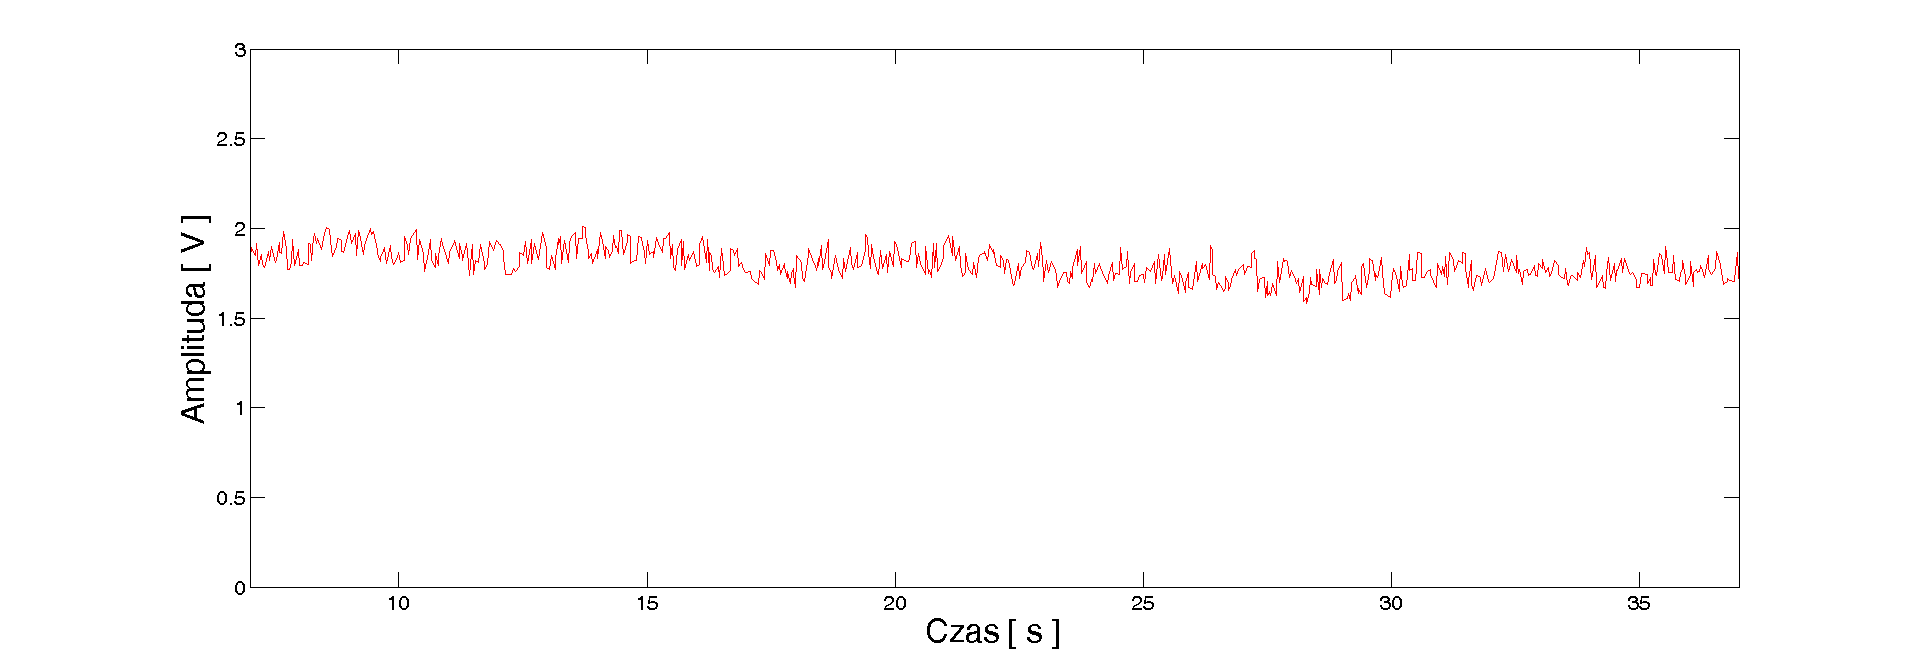
\includegraphics[scale = 0.39]{graphic/filtr1}}
	\caption{Demultipleksowany sygnał diody czerwonej na wyjściu układu próbkująco~-~pamiętającego}
	\label{rys:filtr1}
\end{figure}

Eliminacja szumów  wymaga zastosowania filtru dolnoprzepustowego skutecznie blokującego wszelkie zakłócenia spoza zakresu częstotliwości sygnału użytecznego.
Bliskie sąsiedztwo widma krzywej pletyzmograficznej oraz zakłóceń sieci energetycznej narzuca konieczność stosowania filtrów o~stromych zboczach i~dużej
wartości tłumienia w~pasmie zaporowym. 
Na bazie przeprowadzonych prób i~doświadczeń autor pracy określił wymaganą wartość tłumienia w~paśmie zaporowym na poziomie 50~dB oraz IV rząd filtru. W~celu 
realizacji układu filtru dolnoprzepustowego spełniającego powyższe wymagania zastosowano układ o~topologii Sallen~-~Key~(rys.~\ref{rys:sallenKey}). 
\begin{figure}[!ht]
	\centerline{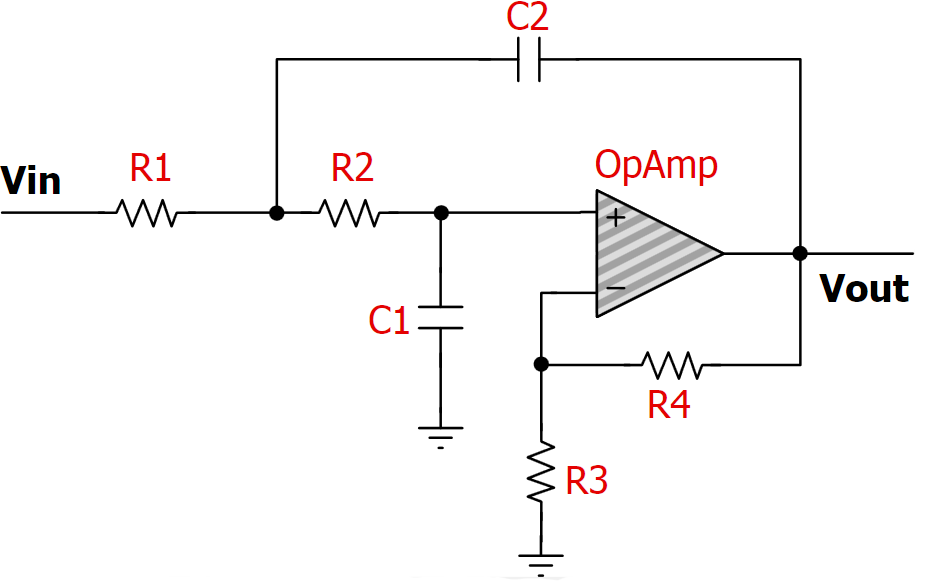
\includegraphics[scale = 0.43]{graphic/sallenKey}}
	\caption{Układ filtru aktywnego o~topologii Sallen~-~Key}
	~\\
	(źródło: na podstawie www.ti.com)
	\label{rys:sallenKey}
\end{figure}

Cechą charakterystyczną zastosowanej konfiguracji jest możliwość implementacji filtrów II rzędu o~różnych charakterystykach przy użyciu pojedynczego wzmacniacza operacyjnego. Filtr IV rzędu uzyskano poprzez 
szeregowe połączenie dwóch segmentów II rzędu. 

Decydujący z~punktu widzenia odpowiedzi filtru na sygnał wejściowy okazał się wybór odpowiedniej charakterystyki amplitudowej. W~fazie projektowania filtru dolnoprzepustowego rozpatrzono charakterystyki 
dolnoprzepustowe Czebyszewa, Butterwortha oraz Bessela. Oceniając odpowiedź układu filtru aktywnego na sygnał analogowy zawierający przebieg fali tętna, parametrem decydującym okazała się podatność poszczególnych 
rodzajów filtru na oscylacje sygnałów wyjściowych (dzwonienie).
Najmniejsze oscylacje zaobserwowano w~filtrach o~charakterystyce Bessela w~przeciwieństwie do układu o~charakterystyce Czebyszewa. Filtr Czebyszewa oraz Butterwortha wykazują znacznie większe nachylenie zboczy 
niż filtr Bessela jednak fakt występowania oscylacji sygnału wyjściowego skutecznie eliminuje możliwość zastosowania filtrów o~charakterystykach tego typu w~układzie pulsoksymetru.
W~układzie pomiarowym zastosowano filtr dolnoprzepustowy o~charakterystyce Bessela w~konfiguracji Sallen~-~Key. Wyznaczenie wartości odpowiednich elementów $R$ i~$C$ dokonano przy użyciu dedykowanego 
oprogramowania FilterPro firmy Texas Instruments~\cite{TI}.\\

Wartości szukanych elementów filtru typu Sallen~-~Key zostały wyznaczone dla następujących parametrów:
\begin{itemize}
	\item Charakterystyka filtru - Bessela
	\item Częstotliwość graniczna dolna - 10~Hz
	\item Częstotliwość graniczna górna - 35~Hz
	\item Maksymalne zafalowania w~paśmie przepustowym - 1~dB
	\item Wartość tłumienia w~paśmie zaporowym - 50~dB
\end{itemize}
\noindent Raport z~symulacji oraz wartości elementów $R$, $C$ zawarto w~dodatku A.\\

Rezultatem filtracji sygnału wyjściowego układu próbkująco~-~pamiętającego jest przebieg na rysunku~\ref{rys:filtr2}.
\begin{figure}[!ht]
	\centerline{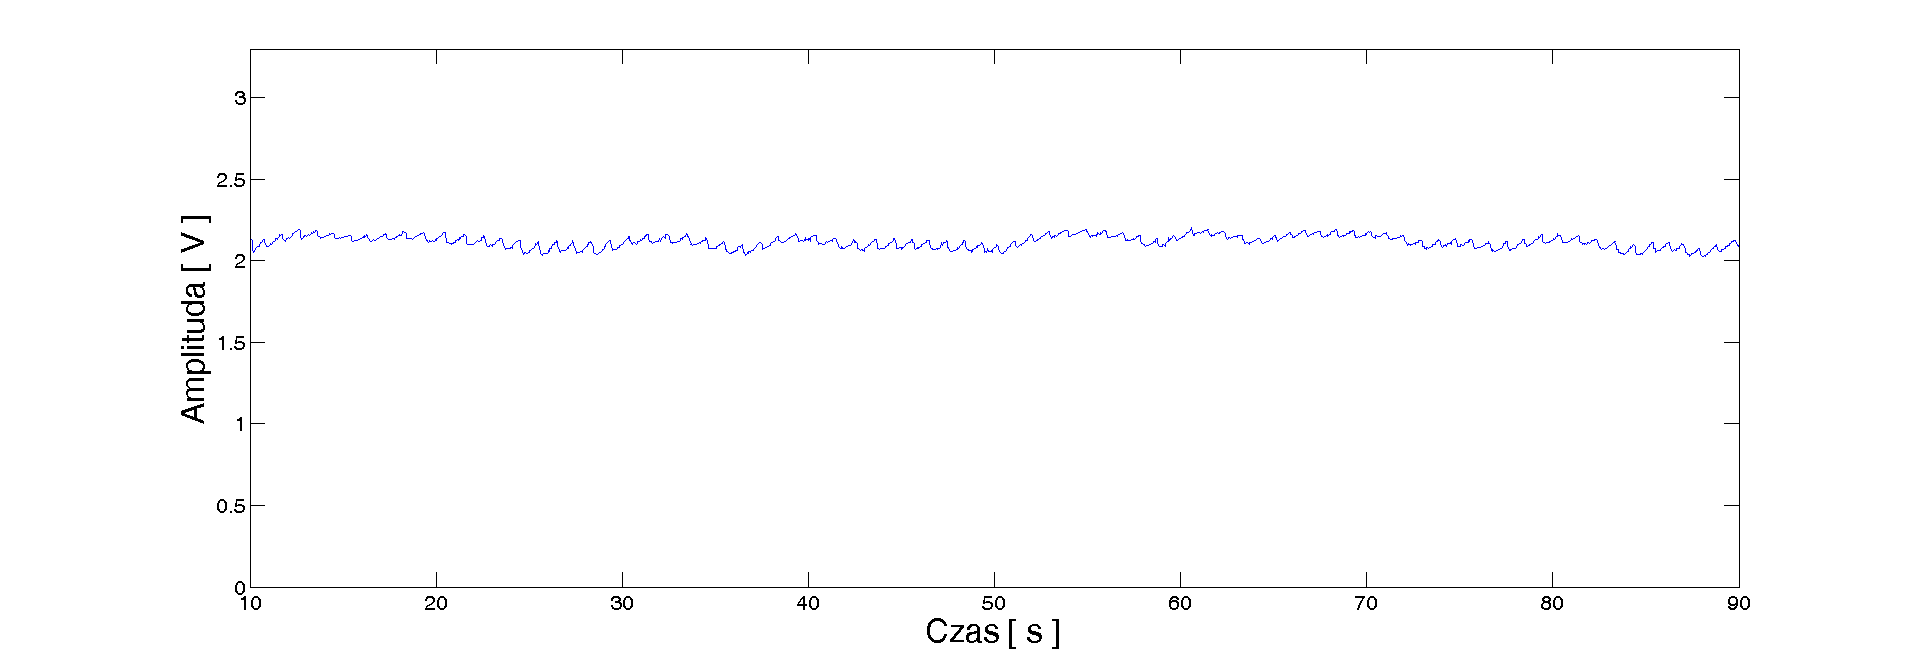
\includegraphics[scale = 0.38]{graphic/filtr2}}
	\caption{Demultipleksowany sygnał diody czerwonej na wyjściu zaprojektowanego filtru dolnoprzepustowego}
	\label{rys:filtr2}
\end{figure}

\subsubsection{Autoregulacja toru pomiarowego}
\label{sec:PID}

Przebieg uzyskany poprzez odfiltrowanie sygnału detektora składa się ze składowej stałej, wolnozmiennego przebiegu krwi żylnej oraz niewielkiego 
przebiegu tętna~(rys.~\ref{rys:calib1}). 
\begin{figure}[ht]
	\centerline{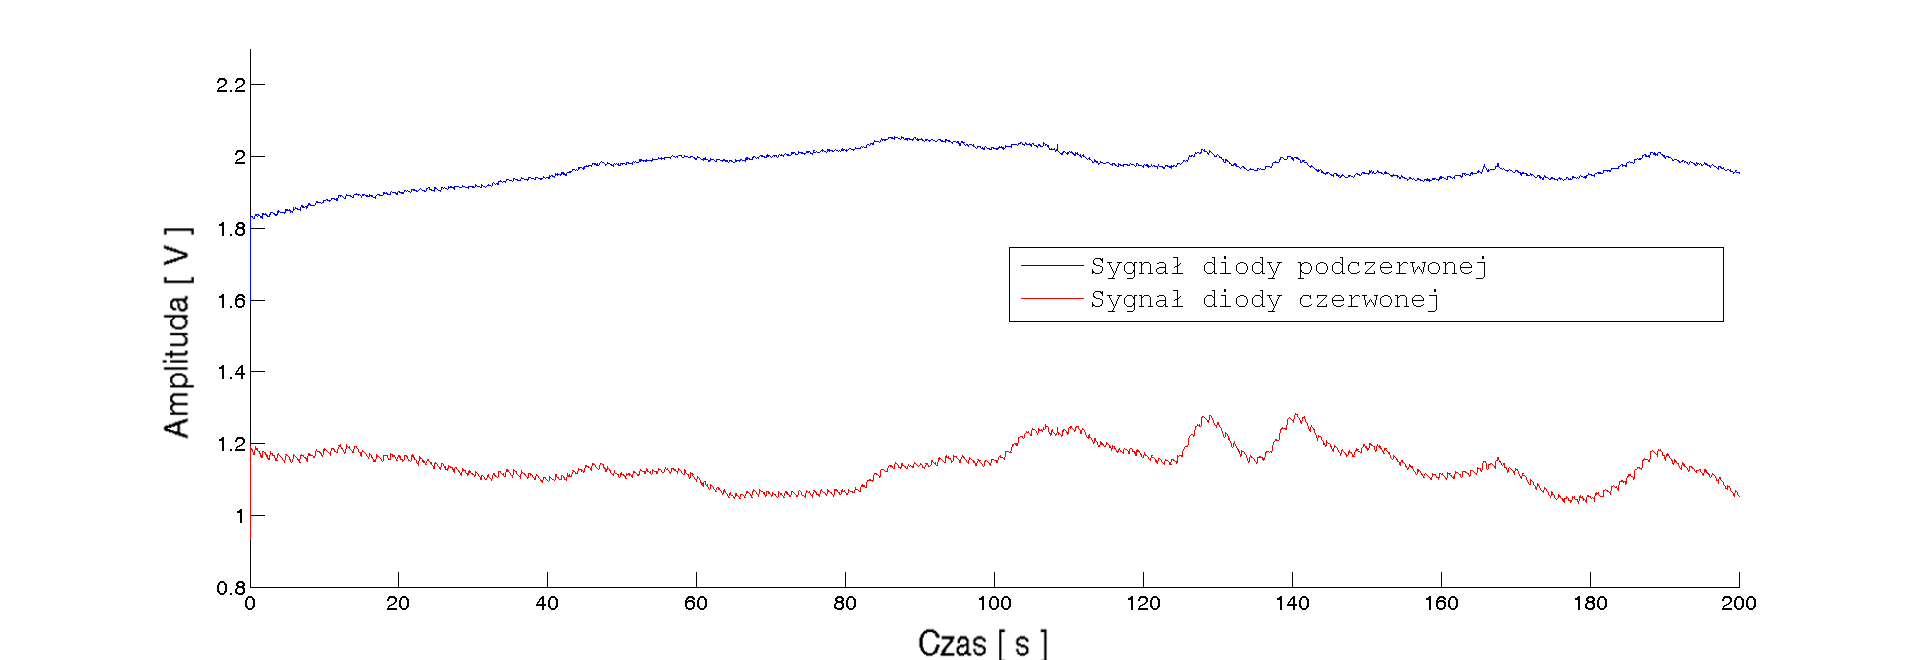
\includegraphics[scale = 0.38]{graphic/calib1}}
	\caption{Sygnał fotodetektora dla dwóch różnych długości fali. Widoczny charakterystyczny sygnał krzywej pletyzmograficznej}
	\label{rys:calib1}
\end{figure}

Wartość składowej DC silnie zależy od grubości, pigmentacji oraz struktury badanego obiektu. W~celu zagwarantowania poprawnej pracy układu 
pomiarowego z~obiektami o~różnych parametrach i~właściwościach, zaproponowano układ autoregulacji toru w~postaci regulatora PID. Pętla 
regulacji obejmuje sterownik źródła promieniowania oraz układ detekcji i~filtrowania sygnału. Układ regulacji kompensuje różnice w~intensywności 
promieniowania diod LED oraz nierównomierność charakterystyki czułości fotodiody. Regulacji podlega wartość składowej stałej sygnału detektora. 

Czas ustalania wartości zadanej zależny jest od współczynników odpowiednich członów regulatora PID. Autor projektu dokonał serii
prób doświadczalnych przy pomocy metod Zieglera~-~Nicholsa, których celem był dobór odpowiednich parametrów regulatora. Zastosowanie metod doświadczalnych,
uwarunkowane zostało brakiem znajomości transmitancji toru pomiarowego. 
Współczynniki regulatora PID wyznaczone na podstawie przyjętych metod nie spełniły założonych wymagań. Rezultaty empirycznej metody doboru parametrów
polegającej na iteracyjnej korekcie współczynników przedstawia rysunek~(rys.~\ref{rys:polka}).
\begin{figure}[ht]
	\centerline{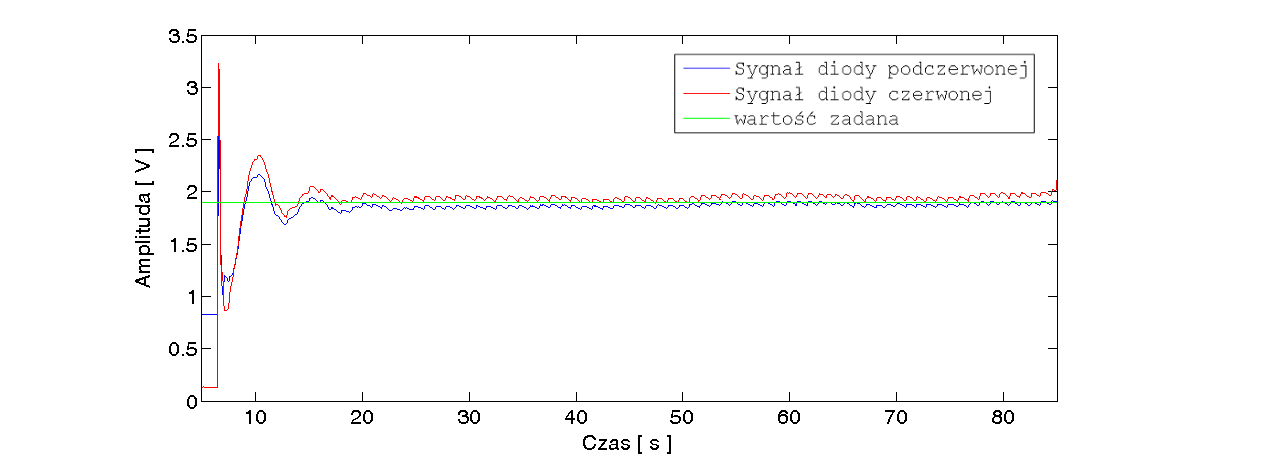
\includegraphics[scale = 0.58]{graphic/pid2}}
	\caption{Przebieg procesu regulacji sygnałów dwóch źródeł promieniowania}
	\label{rys:pid2}
\end{figure}

Alternatywą dla regulatora PID w~układzie pulsoksymetru jest ustalanie wartości zadanej przez stopniową, liniową regulację prądu zasilającego diody 
LED~(rys.~\ref{rys:polka}).
\begin{figure}[!ht]
	\centerline{\includegraphics[scale = 0.38]{graphic/polka}}
	\caption{Proces liniowej regulacji intensywności promieniowania diod LED}
	\label{rys:polka}
\end{figure}

\noindent Czas ustalania wartości zadanej jest znacząco krótszy w~stosunku do czasu ustalania przedstawionego regulatora PID. Regulacja poziomu sygnałów
wyjściowych ma na celu utrzymanie ich na stałym poziomie, co jest niezbędne podczas pomiarów saturacji krwi~(rys.~\ref{rys:polka2}).
\begin{figure}[!ht]
	\centerline{\includegraphics[scale = 0.40]{graphic/polka2}}
	\caption{Proces utrzymywania stałego poziomu sygnałów diod LED}
	\label{rys:polka2}
\end{figure}\\

\section{Wzmacniacz o~regulowanym wzmocnieniu}
\label{sec:PGA}

Obniżenie temperatury otoczenia do niższych wartości od strefy komfortu cieplnego skóry uruchamia mechanizmy adaptacyjne regulacji cieplnej 
ustroju~\cite{SzGa11}. W~pierwszej fazie krótkotrwałego działania zimna skóra jest blada. Skurcz naczyń krwionośnych skóry i~tkanki podskórnej 
występujący pod wpływem niskich temperatur, zmniejsza przepływ krwi i~ogranicza w~ten sposób oddawanie ciepła otoczeniu. Obniżona elastyczność 
tętniczych naczyń krwionośnych skutecznie ogranicza możliwość detekcji fali tętna w~postaci krzywej pletyzmograficznej ($PPG$).

Wpływ temperatury badanego obiektu na amplitudę prądu fotodiody wymusza konieczność zastosowania układu dopasowującego sygnał PPG do zakresu
napięć wejściowych przetwornika analogowo~-~cyfrowego~(rys.~\ref{rys:PGA}).  
\begin{figure}[ht]
	\centerline{\includegraphics[scale = 0.3]{graphic/PGA}}
	\caption{Wzmacniacz operacyjny pracujący jako układ o~zmiennym wzmocnieniu w~konfiguracji nieodwracającej}
	~\\
	(źródło: www.analog.com)
	\label{rys:PGA}
\end{figure}

Wzmacniacz o~regulowanym wzmocnieniu PGA (ang.~Programmable Gain Amplifier) został zrealizowany na bazie wzmacniacza operacyjnego pracującego 
w~konfiguracji nieodwracającej. Regulacja wzmocnienia odbywa się poprzez zastosowanie przestrajanego potencjometru sterowanego cyfrowo.

Wzmocnienie układu wyraża zależność:
\begin{equation}
\label{equ:AMP}
	k_{u} = 1 + \frac{R_{AW}}{R_{2}} 	
\end{equation}

Praca wzmacniacza z~napięciami wejściowymi w~pobliżu dodatniej szyny zasilania wymusza zastosowanie wzmacniacza operacyjnego o~specjalnej konstrukcji
wejściowego stopnia różnicowego (Rail-to-Rail input). Postawione wymagania spełnia wzmacniacz operacyjny typu OPA340. W~roli potencjometru w~pętli 
ujemnego sprzężenia zwrotnego zastosowano potencjometr cyfrowy Microchip MCP41050 o~rezystancji $50~k\Omega$. Sterowanie nastawami potencjometru odbywa
się za pośrednictwem transmisji szeregowej i~interfejsu SPI (ang. Serial Peripherial Interface).

Rezultat zastosowania układu regulowanego wzmacniacza przedstawiono na przebiegu~\ref{rys:wzm}.
\begin{figure}[!h]
	\centerline{\includegraphics[scale = 0.42]{graphic/wzm}}
	\caption{Przebieg krzywej pletyzmograficznej przed i~po wzmocnieniu}
	\label{rys:wzm}
\end{figure}\\

\section{Mikrokontroler sterujący i~wizualizacja wyników}
\label{sec:ARM}

Rdzeń ARM Cortex M3 wraz z~bogatym zestawem układów peryferyjnych, stanowiący układ mikrokontrolera STM32, odpowiedzialny
jest za kontrolę całego procesu pomiarowego. Podstawowe zadania systemu kontrolnego to generowanie sygnałów kluczujących diody LED, 
sterowanie intensywnością światła, regulacja układu PGA oraz obsługa transmisji szeregowej z~nadrzędnym komputerem PC. 
Obliczanie parametrów życiowych odbywa się w~sposób programowy na podstawie danych uzyskanych z~przetworników analogowo~-~cyfrowych.

Konieczność równoczesnej kontroli wielu parametrów procesu pomiarowego wymusza zastosowanie systemu operacyjnego czasu
rzeczywistego. Procedury kontrolno~-~sterujące zrealizowane w~formie odrębnych procesów znacznie ułatwiają ewaluację
kodu źródłowego aplikacji i~proces jego zarządzania. W~pracy zastosowano system operacyjny FreeRTOS w~wersji 7.3.0.\\

Przedstawienie wyników pomiaru częstości akcji serca i~saturacji oraz przebiegi krzywej pletyzmograficznej zrealizowano w~formie
prostej aplikacji w~środowisku LabView~(rys.~\ref{rys:GUI}).\\ 
\begin{figure}[ht]
	\centerline{\includegraphics[scale = 0.55]{graphic/GUI}}
	\caption{Panel czołowy pulsoksymetru w~formie wirtualnego przyrządu LabView}
	\label{rys:GUI}
\end{figure}

Komunikacja z~aplikacją odbywa się poprzez szeregową transmisję na porcie USB. Środowisko LabView umożliwia w~łatwy i~przystępny sposób 
rejestrowanie, analizę oraz wizualizację wyników pomiaru. Dodatkowo istnieje możliwość zapisu uzyskanych danych na dysku twardym komputera 
oraz ich poźniejsze wykorzystanie.

Kompletne urządzenie pomiarowe w~formie obwodu drukowanego PCB wraz z~opisem poszczególnych fragmentów projektu przedstawiono poniżej~(rys.~\ref{rys:PCB}).
\begin{figure}[ht]
	\centerline{\includegraphics[scale = 0.11]{graphic/PCB}}
	\caption{Widok gotowego urządzenia pomiarowego wraz z~opisem najważniejszych elementow układu}
	\label{rys:PCB}
\end{figure}





\renewcommand{\figurename}{Rys.}

\chapter{Badania eksperymentalne i~interpretacja wyników}
\label{cha:test}

\fontsize{14}{15}\selectfont
%----------------------------------------------------------

Silne ukrwienie dłoni umożliwia dokonywanie pomiarów pulsoksymetrem na wszystkich końcówkach palców bez znacznego wpływu na osiągane wyniki 
pomiarów,~np.~\ref{rys:Dlon}.
\begin{figure}[!ht]
	\centerline{\includegraphics[scale = 0.56]{graphic/Dlon}}
	\caption{Układ naczyń krwionośnych dłoni i~palców człowieka}
	\label{rys:Dlon}
	~\\	
	(źródło: Na podstawie \cite{SzGa11})
\end{figure}

W~trakcie mierzenia pulsu zwraca się uwagę na 6 charakterystycznych cech tętna bazując na kształcie krzywej pletyzmograficznej~\cite{SzGa11}.

\noindent \textbf{Częstotliwość} - (liczba wyczuwanych uderzeń w~ciągu minuty), której wartości prawidłowe zależą głównie od wieku. W~czasie badania na uwadze 
należy mieć, że nie należy badać tętna po wysiłku fizycznym (po dużym wysiłku fizycznym częstotliwość może nawet przekraczać 200 uderzeń/min.) lub w~stanie 
silnych przeżyć emocjonalnych. Tętno może być częste (\emph{pulsus frequens}) lub rzadkie (\emph{pulsus rarus}). Przeciętna częstotliwość tętna waha się w~zależności 
od wieku i~wynosi około:
\begin{itemize}
	\item u~płodu: 110-150 [1/min]
	\item u~niemowląt: 130 [1/min]
	\item u~dzieci: 100 [1/min]
	\item u~młodzieży: 85 [1/min]
	\item u~dorosłych: 70 [1/min]
	\item u~ludzi starszych: 60 [1/min]
\end{itemize}
\noindent \textbf{Miarowość} - tętno jest miarowe (\emph{pulsus regularis}) jeśli wszystkie uderzenia wykazują jednakową siłę, a~odstępy między nimi są jednakowe, 
w~przeciwnym razie mówimy o~tętnie niemiarowym (\emph{pulsus irregularis}).

\noindent \textbf{Wypełnienie} - określa wysokość fali tętna i~zależy od wypełnienia tętnicy krwią, co z~kolei zależy od rzutu serca. Tętno może być wysokie (duże) 
(\emph{pulsus altus, pulsus magnus}), małe (\emph{pulsus parvus}), nitkowate, równe (\emph{pulsus equalis}), nierówne i~dziwaczne (\emph{pulsus paradoxus}).

\noindent \textbf{Napięcie} - cecha tętna będąca wyrazem ciśnienia tętniczego. Tętno może być twarde (\emph{pulsus durus}), miękkie (\emph{pulsus mollis}) bądź dwubitne.

\noindent \textbf{Chybkość} - zależy od szybkości wypełniania się tętnicy i~zapadania jej światła w~okresie jednego cyklu pracy serca. Zależy od prędkości przepływu krwi 
i~podatności ściany tętnic. Tętno może być chybkie (\emph{pulsus celer}) lub leniwe (\emph{pulsus tardus}).

\noindent \textbf{Symetria} - fizjologicznie tętno powinno być takie samo po lewej i~po prawej stronie ciała.

Średnie tętno spoczynkowe zależy przede wszystkim od wieku i~stopnia wytrenowania,~np.~\ref{rys:TetnoTabela}.
\begin{figure}[ht]
	\centerline{\includegraphics[scale = 1.1]{graphic/TetnoTabela}}
	\caption{Zależność tętna spoczynkowego od wieku, płci i~kondycji organizmu}
	\label{rys:TetnoTabela}
	~\\	
	(źródło: Na podstawie \cite{SzGa11})
\end{figure}


\section{Pomiar częstości akcji serca}
\label{sec:Puls}

Pomiaru tętna, czyli częstości skurczów serca na minutę dokonuje się analizując przebieg krzywej pletyzmograficznej.
Charakterystyczny zmienny przebieg krzywej $PPG$ jest skutkiem zmian objętości naczyń krwionośnych pod wpływem przepływającej krwi pompowanej przez mięsień 
sercowy. Skurcze komór serca zwiększające objętość naczyń tętniczych są widoczne jako lokalne ekstrema krzywej pletyzmograficznej~(rys.~\ref{rys:MAX}).
\begin{figure}[!ht]
	\centerline{\includegraphics[scale = 0.58]{graphic/MAX}}
	\caption{Moment skurczu komór serca zarejestrowany na przebiegu krzywej pletyzmograficznej $PPG$. Pomiar dokonany zaprojektowanym pulsoksymetrem}
	\label{rys:MAX}
\end{figure}

Praktycznie, chwilowa wartość częstości akcji serca wyznaczana przez pulsoksymetr obliczana jest z~następującej zależności:
\begin{equation}
	BPM = \frac{60}{T}~~[1/min]
\end{equation}
gdzie:\\
$T$ - okres pomiędzy kolejnymi uderzeniami serca w~sekundach.

Poprawności pomiaru zaprojektowanego pulsoksymetru autor dokonał poprzez porównanie uzyskanych wyników z~wynikami komercyjnego ciśnieniomierza typu Hartmann Tensoval Mobil,
wyposażonego w~funkcję pomiaru tętna~(rys.~\ref{rys:tensoval}).
\begin{figure}[!ht]
	\centerline{\includegraphics[scale = 0.38]{graphic/tensoval}}
	\caption{Ciśnieniomierz nadgarstkowy Tensoval Mobil firmy Hartmann}
	~\\
	(źródło: http://www.tensoval.pl)
	\label{rys:tensoval}
\end{figure}

Analiza porównawcza ma na celu stwierdzenie poprawności wyników uzyskanych podczas pomiaru tętna przy użyciu zaprojektowanego pulsoksymetru. Urządzenie
umożliwia pomiar chwilowej częstości skurczów komór serca. Punkt odniesienia stanowi wynik pomiaru ciśnieniomierza nadgarstkowego, którego wynik 
określa średnią częstotliwość uderzeń serca w~ciągu trwania pomiaru ciśnienia.

\noindent Wynik pomiaru częstości akcji serca u~pacjenta w~stanie spoczynku przedstawia przebieg na rysunku~\ref{rys:Tetno_D_2}.
\begin{figure}[!h]
	\centerline{\includegraphics[scale = 0.63]{graphic/Tetno_D_2}}
	\caption{Pomiar chwilowego oraz średniego tętna pacjenta w~stanie spoczynku}
	\label{rys:Tetno_D_2}
\end{figure}

\noindent Chwilowa wartość tętna zawiera się w~zakresie dopuszczalnych wartości dla człowieka zdrowego wynoszącym od 60 do 80 uderzeń na minutę. 
Średnia wartość częstotliwości pulsoksymetru pokrywa się z~wynikiem uzyskanym przy pomocy urządzenia Tensoval.
\noindent Wzmożona praca mięśni organizmu w~trakcie wysiłku fizycznego wymaga dostarczenia większej ilości tlenu do komórek ciała, co skutkuje zwiększeniem
częstotliwości skurczów serca~(rys.~\ref{rys:Tetno_D_1}). 
\begin{figure}[!ht]
	\centerline{\includegraphics[scale = 0.62]{graphic/Tetno_D_1}}
	\caption{Pomiar chwilowego oraz średniego tętna pacjenta w~trakcie wysiłku fizycznego}
	\label{rys:Tetno_D_1}
\end{figure}

\noindent Podczas weryfikacji poprawności pomiarów pulsoksymetru dokonano serii pomiarów częstości akcji serca u~pacjentów
w różnych przedziałach wiekowych. Wyniki pomiarów przedstawiają przebiegi z~rysunków~\ref{rys:2L}, \ref{rys:25L}, \ref{rys:30L},
\ref{rys:50-60M}, \ref{rys:50-60K} oraz \ref{rys:90L}.
\begin{figure}[!ht]
	\centerline{\includegraphics[scale = 0.6]{graphic/2L}}
	\caption{Pomiar chwilowego oraz średniego tętna pacjenta w~wieku 2 lat (chłopiec)}
	\label{rys:2L}
\end{figure}

\noindent Średnia wartość tętna u~dziecka jest zdecydowanie wyższa niż u~młodzieży oraz osób starszych i~zawiera się w~granicach 
80~-~90~[1/min]. 
\begin{figure}[!h]
	\centerline{\includegraphics[scale = 0.6]{graphic/25L}}
	\caption{Pomiar chwilowego oraz średniego tętna pacjenta w~wieku 25 lat (mężczyzna)}
	\label{rys:25L}
\end{figure}
\newpage
\begin{figure}[!ht]
	\centerline{\includegraphics[scale = 0.6]{graphic/30L}}
	\caption{Pomiar chwilowego oraz średniego tętna pacjenta w~wieku 30 lat (mężczyzna)}
	\label{rys:30L}
\end{figure}
\begin{figure}[!hb]
	\centerline{\includegraphics[scale = 0.6]{graphic/50-60M}}
	\caption{Pomiar chwilowego oraz średniego tętna pacjenta w~przedziale wiekowym 50~-~60 lat (mężczyzna)}
	\label{rys:50-60M}
\end{figure}
\newpage
\begin{figure}[!ht]
	\centerline{\includegraphics[scale = 0.61]{graphic/50-60K}}
	\caption{Pomiar chwilowego oraz średniego tętna pacjenta w~przedziale wiekowym 50~-~60 lat (kobieta)}
	\label{rys:50-60K}
\end{figure}

\begin{figure}[!hb]
	\centerline{\includegraphics[scale = 0.61]{graphic/90L}}
	\caption{Pomiar chwilowego oraz średniego tętna pacjenta w~wieku 90 lat (kobieta)}
	\label{rys:90L}
\end{figure}
\newpage

Wynik testu dotyczącego powtarzalności uzyskiwanych wyników przedstawiono na rysunku~\ref{rys:proba}.
Przeprowadzone pomiary potwierdzają wpływ wieku i~kondycji pacjenta na osiągane wyniki częstości skurczów serca. Jednocześnie
poprzez analizę porównawczą dowiedziono poprawności pomiarów tętna przy użyciu zaprojektowanego pulsoksymetru.
Odstępności od wyników urządzenia Tensoval spowodowane są umiejscowieniem sondy pomiarowej, metodą pomiaru oraz sposobem
przedstawiania wyników (uśrednianie).
\begin{figure}[!h]
	\centerline{\includegraphics[scale = 0.6]{graphic/proba}}
	\caption{Wartość tętna pacjenta podczas kolejnych prób pomiarowych}
	\label{rys:proba}
\end{figure}

\section{Pomiar wysycenia krwi tętniczej tlenem ($SpO2$)}
\label{sec:Saturacja}

Odmienne właściwości optyczne oksyhemoglobiny oraz hemoglobiny, powodujące różny stopień absorpcji promieniowania przez krew,
powodują detekcję sygnału krzywej pletyzmograficznej o~różnej amplitudzie~(rys.~\ref{rys:PPG1}).
\begin{figure}[!ht]
	\centerline{\includegraphics[scale = 0.6]{graphic/PPG1}}
	\caption{Przebieg krzywej PPG dla promieniowania 660~nm oraz 940~nm}
	\label{rys:PPG1}
\end{figure}

Pomiarów wysycenia krwi tętniczej tlenem dokonano metodą wyliczania współczynnika R zależnego od amplitudy sygnału $PPG$ podczas
skurczu i~rozkurczu komór serca~(wzór~\ref{sec:Fotopletyzmografia}). Zaprojektowany pulsoksymetr wykorzystuje następującą zależność 
saturacji krwi w~funkcji współczynnika R~(rys.~\ref{rys:curve}). 
\begin{figure}[!h]
	\centerline{\includegraphics[scale = 0.51]{graphic/curve}}
	\caption{Empiryczna krzywa kalibracji pulsoksymetru}
	\label{rys:curve}
	~\\	
	(źródło: Na podstawie \cite{Katja:2011})
\end{figure}

\noindent Krzywa kalibracji została stworzona na bazie doświadczeń prowadzonych w~laboratorium na próbkach krwi o~różnych stopniach 
natlenowania (in vitro)~\cite{Katja:2011}.

Autor porównał parametry osiągane za pomocą zaprojektowanego urządzenia z~wynikiem komercyjnego pulsoksymetru Respironix Novametrix COSMO, co 
stanowi podstawę do stwierdzenia poprawności funkcjonowania urządzenia~(rys.~\ref{rys:COSMO}).
\begin{figure}[!ht]
	\centerline{\includegraphics[scale = 0.80]{graphic/COSMO}}
	\caption{Pulsoksymetr szpitalny Respitronix Novametrix COSMO}
	\label{rys:COSMO}
	~\\
	(źródło: http://www.somatechnology.com)
\end{figure}
Poprawny parametr SpO2 zawiera się w~granicach 95\%~–~99\%~\cite{SzGa11}. Pomiar wysycenia krwi tlenem badanego aparatu w~stosunku 
do pomiaru urządzeniem szpitalnym przedstawiono na rysunku~\ref{rys:Saturacja1}.
\begin{figure}[!ht]
	\centerline{\includegraphics[scale = 0.60]{graphic/Saturacja1}}
	\caption{Zestawienie uzyskanych wyników saturacji przy użyciu dwóch różnych aparatów pomiarowych}
	\label{rys:Saturacja1}
\end{figure}

Uzyskane wyniki wykazują zbieżność pomiarów zaprojektowanego urządzenia z~pomiarem wykonanym aparatami komercyjnymi. Wartości saturacji zdrowego organizmu
oscylują z~niewielką amplitudą wokół wartości 97~\%, mieszczącej się w~dopuszczalnym zakresie.

W~celu stwierdzenia zgodności pomiarów wartości saturacji należy przeprowadzić serię pomiarów na grupie pacjentów o~zróżnicowanym stopniu
natlenowania krwi tętniczej. Zatrucia tlenkiem węgla, długotrwałe palenie tytoniu, anemia, sinica lub terapia tlenowa to główne powody 
zmiany stopnia natlenowania krwi. Trudności z~dostępem do odpowiedniej grupy pacjentów wymuszają przeprowadzenie pomiarów weryfikacyjnych 
na osobach zdrowych. Podczas pomiarów saturacji dokonano zróżnicowania wyników ze względu na wiek badanych osób, np.~\ref{rys:Sat25}, 
\ref{rys:Sat30K}, \ref{rys:Sat30M}, \ref{rys:Sat50M} oraz \ref{rys:Sat90}.\\
\begin{figure}[!h]
	\centerline{\includegraphics[scale = 0.63]{graphic/Sat25}}
	\caption{Pomiar saturacji chwilowej - pacjent w~wieku 25 lat (mężczyzna)}
	\label{rys:Sat25}
\end{figure}
\newpage
\begin{figure}[!h]
	\centerline{\includegraphics[scale = 0.63]{graphic/Sat30K}}
	\caption{Pomiar saturacji chwilowej - pacjent w~wieku 30 lat (kobieta)}
	\label{rys:Sat30K}
\end{figure}
\begin{figure}[!h]
	\centerline{\includegraphics[scale = 0.63]{graphic/Sat30M}}
	\caption{Pomiar saturacji chwilowej - pacjent w~wieku 30 lat (mężczyzna)}
	\label{rys:Sat30M}
\end{figure}
\newpage
\begin{figure}[!h]
	\centerline{\includegraphics[scale = 0.61]{graphic/Sat50M}}
	\caption{Pomiar saturacji chwilowej - pacjent w~wieku 59 lat (mężczyna)}
	\label{rys:Sat50M}
\end{figure}
\begin{figure}[!h]
	\centerline{\includegraphics[scale = 0.61]{graphic/Sat90}}
	\caption{Pomiar saturacji chwilowej - pacjent w~wieku 90 lat (kobieta)}
	\label{rys:Sat90}
\end{figure}

\noindent Wyniki testów weryfikujących powtarzalność uzyskiwanych wyników przedstawia rysunek~\ref{rys:SatProba}. Spadek wartości
saturacji będący skutkiem zmniejszania dopływu tlenu do płuc zaobserwowano podczas testu polegającego na długotrwałym wstrzymywaniu
oddechu~(rys.~\ref{rys:spadek}).
\begin{figure}[!ht]
	\centerline{\includegraphics[scale = 0.58]{graphic/SatProba}}
	\caption{Wartość saturacji wyznaczona dla pacjenta podczas kolejnych prób pomiarowych}
	\label{rys:SatProba}
\end{figure}\\
\begin{figure}[!ht]
	\centerline{\includegraphics[scale = 0.38]{graphic/spadek}}
	\caption{Wpływ wstrzymywania oddechu na wskaźnik wysycenia krwi tętniczej tlenem}
	\label{rys:spadek}
\end{figure}\\

Pomiary saturacji krwi tętniczej wykazały brak zależności wartości wskaźnika SpO2 od wieku badanego pacjenta. Zaobserwowano
niewielki rozrzut parametru wokół wartości 96\%, która zawarta jest w~dopuszczalnym zakresie.   
\noindent Bazując na przykładowej, empirycznej krzywej kalibracyjnej dokonano serii pomiarów, których wyniki pokrywają się
z~wartościami oczekiwanymi. W~celu kompletnej kalibracji zaprojektowanego urządzenia, należy dokonać
analizy gazometrycznej krwi o~różnym stopniu wysycenia tlenem, co posłuży do określenia krzywej kalibracji konkretnego 
aparatu pomiarowego. 

\renewcommand{\figurename}{Rys.}

\chapter{Podsumowanie}
\label{cha:podsumowanie}

Po gruntownym zapoznaniu się z~wybranymi zagadnieniami biofizyki i biochemii dotyczącymi właściwości optycznych zbiorów komórek organizmu, dokonano 
analizy możliwości wykorzystania interakcji światło~-~tkanka w~detekcji parametrów określających stan układu krążeniowo~-~oddechowego. 
Przegląd zjawisk fizycznych zachodzących wewnątrz oraz na granicach struktur tkankowych wraz z~wiedzą na temat funkcji oraz roli krwioobiegu 
i~układu oddechowego posłużyły jako podstawa do analizy wykorzystania praw optyki w~diagnostyce medycznej. Idea oraz metodyka przeprowadzania 
pomiarów bazujących na transluminacji promieniowaniem w~postaci światła, pozwoliła na wyznaczenie zależności pomiędzy cechami uzyskanego 
sygnału a~poszukiwanymi wskaźnikami częstości akcji serca i~saturacji. 

Wynikiem pracy jest przenośny układ elektroniczny umożliwiający pomiar wybranych parametrów krwi takich, jak: tętno i saturacja. W~ramach pracy 
wykonany został kompletny system pomiarowy złożony z~analogowego toru przetwarzania sygnału $PPG$ oraz cyfrowego modułu kontrolno~-~sterującego 
w~postaci mikrokontrolera STM32. Całość aparatu pomiarowego została zrealizowana w formie obwodu drukowanego PCBi, gwarantującego integralność 
i~niezawodność pracy urządzenia. Kontrolę nad procesem pomiarowym sprawuje aplikacja mikrokontrolera napisana w~języku C przy wsparciu systemu 
operacyjnego czasu rzeczywistego FreeRTOS. Zastosowanie systemu operacyjnego znacznie ułatwiło proces tworzenia i~ewaluacji kodu źródłowego aplikacji, 
umożliwiając równocześnie łatwe wprowadzenie nowych funkcjonalności. Pulsoksymetr zasilany jest z~zewnętrznego źródła napięcia 5~V w~postaci zasilacza oraz
posiada możliwość przesyłania danych do nadrzędnego komputera PC interfejsem USB. Wizualizacja wyników pomiaru wraz z~przebiegiem krzywej
pletyzmograficznej zrealizowana została w formie prostej aplikacji w środowisku LabView.

Końcowa faza testowania i~kalibracji urządzenia wykazała dużą zbieżność mierzonych wartości z~wynikami komercyjnych urządzeń szpitalnych wykorzystywanych
podczas testów porównawczych. Testy pomiaru tętna oraz stopnia wysycenia krwi tętniczej tlenem wykonane zostały na grupie zdrowych osób 
w zróżnicowanych przedziałach wiekowych. Ostatecznie stwierdzono poprawność funkcjonowania aparatu pomiarowego przy założeniu spełnienia
określonych warunków przeprowadzanego pomiaru. 

\subsubsection{Dalsze kierunki rozwoju}
\label{subsubsec:Rozwoj}

Podstawowy zakres funkcji zaprojektowanego pulsoksymetru obejmuje pomiar wartości saturacji oraz tętna wraz z~wizualizacją wyników. 
W~trosce o~dalszą ewaluację projektu układ wyposażono w złącze wyświetlacza LCD $3.2"$ SSD1298 z~panelem dotykowym i~złączem karty SD. W~celu zapewnienia 
pełnej mobilności urządzenia warto zaimplementować tryb zasilania bateryjnego. Współczesne technologie miniaturyzacji elementów i~układów 
elektronicznych umożliwiają zmniejszenie wymiarów aparatu pomiarowego do rozmiarów porównywalnych z~wymiarami sondy napalcowej. Miniaturyzacja 
pulsoksymetru oraz wyposażenie układu w możliwość transmisji bezprzewodowej pozwolą na włączenie urządzenia do sieci zdalnego monitorowania 
pacjenta WBAN (ang.~Wireless Body Area Network). Warunkiem koniecznym jest opracowanie systemu eliminacji zakłóceń i artefaktów będących skutkiem
ruchów pacjenta.



\renewcommand{\figurename}{Rys.}

\chapter*{Dodatek A}
\label{cha:dodatekA}
\addcontentsline{toc}{chapter}{Dodatek A}


\fontsize{14}{15}\selectfont
%----------------------------------------------------------
\begin{itemize}
	\item \textbf{Schematy elektryczne pulsoksymetru}
		\begin{itemize}
			\item Schemat~I  - układ sterowania intensywnością promieniowania diod LED,
			\item Schemat~II - konwerter prąd~-~napięcie i~układ  próbkująco~-~pamiętający,
			\item Schemat III - filtr dolnoprzepustowy Sallen~-~Key IV~rzędu,
			\item Schemat IV - mikrokontroler STM32, interfejs USB,
			\item Schemat V  - układ zasilania, interfejs JTAG .
		\end{itemize}
	\item \textbf{Projekt PCB}
		\begin{itemize}
			\item Warstwa TOP
			\item Warstwa BOTTOM
		\end{itemize}
	\item \textbf{Spis elementów w formie raportu BOM}
	\item \textbf{Raport symulacji filtru Bessela FilterPro TI}
\end{itemize}

\includepdf[pages={1}, landscape]{graphic/SchematI.pdf}
\includepdf[pages={1}, landscape]{graphic/SchematII.pdf}
\includepdf[pages={1}, landscape]{graphic/SchematIII.pdf}
\includepdf[pages={1}, landscape]{graphic/SchematIV.pdf}
\includepdf[pages={1}, landscape]{graphic/SchematV.pdf}

\newpage
\begin{figure}[!ht]
	\centerline{\includegraphics[scale = 0.26]{graphic/top.png}}
	\caption{Warstwa TOP (odbicie lustrzane)}
	\label{rys:Dlon}
\end{figure}
\begin{figure}[!ht]
	\centerline{\includegraphics[scale = 0.26]{graphic/bottom.png}}
	\caption{Warstwa BOTTOM}
	\label{rys:Dlon}
\end{figure}
\newpage

\includepdf[pages={1,2}]{graphic/BOM.pdf}
\includepdf[pages={1,2}]{graphic/designreport.pdf}


\renewcommand{\figurename}{Rys.}

\chapter*{Dodatek B}
\label{cha:dodatekB}
\addcontentsline{toc}{chapter}{Dodatek B}

\fontsize{14}{15}\selectfont
%----------------------------------------------------------
\section*{\LARGE Zawartość nośnika DVD}
\label{sec:Schematy}



\cleardoublepage
\phantomsection
\addcontentsline{toc}{chapter}{Bibliografia}

\begingroup
\large
\bibliographystyle{ieeetr}
\bibliography{bibliografia}

\cleardoublepage
\phantomsection
\addcontentsline{toc}{chapter}{Spis rysunków}
\listoffigures
\endgroup
\renewcommand{\figurename}{Fig.}

%\addcontentsline{toc}{chapter}{Spis tabel}

\end{document}
